% Soubory musí být v kódování, které je nastaveno v příkazu \usepackage[...]{inputenc}

\documentclass[% Základní nastavení
	%draft,				% Testovací překlad
	12pt,				% Velikost základního písma je 12 bodů
	a4paper,			% Formát papíru je A4
	%oneside,			% Jednostranný tisk
	twoside,			% Dvoustranný tisk (kapitoly a další důležité části tedy začínají na lichých stranách)
	unicode,			% Záložky a metainformace ve výsledném  PDF budou v kódování unicode
]{report}				% Dokument třídy 'zpráva', vhodná pro sazbu závěrečných prací s kapitolami

% Kódování zdrojových souborů je UTF-8
\usepackage[utf8]
	{inputenc}			% Balíček pro nastavení kódování zdrojových souborů

% přetypuje nadpisy všech úrovní na bezpatkové, kromě \chapter, která je přenastavena zvlášť v thesis.sty
\usepackage{sectsty}
	\allsectionsfont{\sffamily}

\usepackage{graphicx}	% Balíček 'graphicx' pro vkládání obrázků
						% Nutné pro vložení logotypů školy a fakulty

\usepackage[			% Balíček 'acronym' pro sazby zkratek a symbolů
	nohyperlinks		% Nebudou tvořeny hypertextové odkazy do seznamu zkratek
]{acronym}
						% Nutné pro použití prostředí 'acronym' balíčku 'thesis'

\usepackage[
	breaklinks=true,	% Hypertextové odkazy mohou obsahovat zalomení řádku
	hypertexnames=false	% Názvy hypertext. odkazů budou tvořeny nezávisle na názvech TeXu
]{hyperref}				% Balíček 'hyperref' pro sazbu hypertextových odkazů
						% Nutné pro použití příkazu 'pdfsettings' balíčku 'thesis'

\usepackage{pdfpages}	% Balíček umožňující vkládat stránky z PDF souborů
						% Nutné při vkládání titulních listů a zadání přímo
						% ve formátu PDF z informačního systému

\usepackage{enumitem}	% Balíček pro nastavení mezerování v odrážkách
	\setlist{topsep=0pt,partopsep=0pt,noitemsep} % konkrétní nastavení

\usepackage{cmap}		% Balíček cmap zajišťuje, že PDF vytvořené `pdflatexem' je
						% plně "prohledávatelné" a "kopírovatelné"

%\usepackage{upgreek}	% Balíček pro sazbu stojatých řeckých písmem
						%% např. stojaté pí: \uppi
						%% např. stojaté mí: \upmu (použitelné třeba v mikrometrech)
						%% pozor, grafická nekompatibilita s fonty typu Computer Modern!

\usepackage{amsmath}	% balíček pro sadu náročnější matematiky

\usepackage{placeins}	% Balíček pro zajištění, že se obrázky a tabulky nebudou posouvat
						% za kapitolu, ve které jsou uvedeny

\usepackage{dirtree}	% sazba adresářové struktury
						% vhodné pro prezentaci obsahu elektronické přílohy (např. CD)

\usepackage[formats]{listings}	% Balíček pro sazbu zdrojových textů
\lstset{% nastavení
% Definice jazyka použitého ve výpisech
	%language=[LaTeX]{TeX},	% LaTeX
	%language={Matlab},		% Matlab
	% language={C},			% jazyk C
	language={Python},		% Python
	basicstyle=\ttfamily,	% definice základního stylu písma
	tabsize=2,				% definice velikosti tabulátoru
	inputencoding=utf8,		% pro soubory uložené v kódování UTF-8
	columns=fixed,			% fixed nebo flexible,
	fontadjust=true			% licovani sloupcu
	extendedchars=true,		% podpora nestandardních znaků
% Definice symbolů s diakritikou
	literate=
	{á}{{\'a}}1
	{č}{{\v{c}}}1
	{ď}{{\v{d}}}1
	{é}{{\'e}}1
	{ě}{{\v{e}}}1
	{í}{{\'i}}1
	{ň}{{\v{n}}}1
	{ó}{{\'o}}1
	{ř}{{\v{r}}}1
	{š}{{\v{s}}}1
	{ť}{{\v{t}}}1
	{ú}{{\'u}}1
	{ů}{{\r{u}}}1
	{ý}{{\'y}}1
	{ž}{{\v{z}}}1
	{Á}{{\'A}}1
	{Č}{{\v{C}}}1
	{Ď}{{\v{D}}}1
	{É}{{\'E}}1
	{Ě}{{\v{E}}}1
	{Í}{{\'I}}1
	{Ň}{{\v{N}}}1
	{Ó}{{\'O}}1
	{Ř}{{\v{R}}}1
	{Š}{{\v{S}}}1
	{Ť}{{\v{T}}}1
	{Ú}{{\'U}}1
	{Ů}{{\r{U}}}1
	{Ý}{{\'Y}}1
	{Ž}{{\v{Z}}}1
}

%%%%%%%%%%%%%%%%%%%%%%%%%%%%%%%%%%%%%%%%%%%%%%%%%%%%%%%%%%%%%%%%%
%%%%%%      Definice informací o dokumentu             %%%%%%%%%%
%%%%%%%%%%%%%%%%%%%%%%%%%%%%%%%%%%%%%%%%%%%%%%%%%%%%%%%%%%%%%%%%%

% do tohoto souboru doplňte údaje o sobě, druhu práce, názvu...
% V tomto souboru se nastavují téměř veškeré informace, proměnné mezi studenty:
% jméno, název práce, pohlaví atd.
% Tento soubor je SDÍLENÝ mezi textem práce a prezentací k obhajobě = netřeba něco nastavovat na dvou místech.

\usepackage[
%%% Z následujících voleb jazyka lze použít pouze jednu
	czech-english,		% originální jazyk je čeština, překlad je anglicky (výchozí)
	%english-czech,		% originální jazyk je angličtina, překlad je česky
	%slovak-english,	% originální jazyk je slovenština, překlad je anglicky
	%english-slovak,	% originální jazyk je angličtina, překlad je slovensky
%
%%% Z následujících voleb typu práce lze použít pouze jednu
	%semestral,			% semestrální práce (výchozí)
	bachelor,			% bakalářská práce
	%master,			% diplomová práce
	%treatise,			% pojednání o disertační práci
	%doctoral,			% disertační práce
%
%%% Z následujících voleb zarovnání objektů lze použít pouze jednu
	%left,				% rovnice a popisky plovoucích objektů budou zarovnány vlevo
	center,				% rovnice a popisky plovoucích objektů budou zarovnány na střed (vychozi)
%
%%% Níže uvedený přepinač 'electronic' lze použít pro generování elektronické verze práce; pokud je aktivní, vnější a vnitřní okraj sazebního obrazce budou shodné pro liché i sudé stránky.
% Pozor, neplést si s volbou oneside/twoside!
% Pozor, pro tiskovou verzi nechejte vypnuté!
	%electronic
]{thesis}				% Balíček pro sazbu studentských prací


%%% Jméno a příjmení autora ve tvaru
% [tituly před jménem]{Křestní}{Příjmení}[tituly za jménem]
% Pokud osoba nemá titul před/za jménem, smažte celý řetězec '[...]'
\author{Petr}{Šimčák}

%%% Identifikační číslo autora (VUT ID)
\butid{226320}

%%% Pohlaví autora/autorky
% (nepoužije se ve variantě english-czech ani english-slovak)
% Číselná hodnota: 1 = žena, 0 = muž
\gender{0}

%%% Jméno a příjmení vedoucího/školitele včetně titulů
% [tituly před jménem]{Křestní}{Příjmení}[tituly za jménem]
% Pokud osoba nemá titul před/za jménem, smažte celý řetězec '[...]'
\advisor[doc.\ Ing.]{Jiří}{Kozumplík}[CSc.]

%%% Jméno a příjmení oponenta včetně titulů
% [tituly před jménem]{Křestní}{Příjmení}[tituly za jménem]
% Pokud osoba nemá titul před/za jménem, smažte celý řetězec '[...]'
% Nastavení oponenta se uplatní pouze v prezentaci k obhajobě;
% v případě, že nechcete, aby se na titulním snímku prezentace zobrazoval oponent, pouze příkaz zakomentujte;
% u obhajoby semestrální práce se oponent nezobrazuje (jelikož neexistuje)
% U dizertační práce jsou typicky dva až tři oponenti. Pokud je chcete mít na titulním slajdu, prosím ručně odkomentujte a upravte jejich jména v definici "VUT title page" v souboru thesis.sty.
\opponent[doc.\ Mgr.]{Křestní}{Příjmení}[Ph.D.]

%%% Název práce
%  Parametr ve složených závorkách {} je název v originálním jazyce,
%  parametr v hranatých závorkách [] je překlad (podle toho jaký je originální jazyk).
%  V případě, že název Vaší práce je dlouhý a nevleze se celý do zápatí prezentace, použijte příkaz
%  \def\insertshorttitle{Zkác.\ náz.\ práce}
%  kde jako parametr vyplníte zkrácený název. Pokud nechcete zkracovat název, budete muset předefinovat,
%  jak se vytváří patička slidu. Viz odkaz: https://bit.ly/3EJTp5A
\title[Heart Rate Estimation from the PPG Signals]{Odhad tepové frekvence ze signálů PPG}

%%% Označení oboru studia
%  Parametr ve složených závorkách {} je název oboru v originálním jazyce,
%  parametr v hranatých závorkách [] je překlad
\specialization[Sport technology]{Sportovní technologie}

%%% Označení ústavu
%  Parametr ve složených závorkách {} je název ústavu v originálním jazyce,
%  parametr v hranatých závorkách [] je překlad
%\department[Department of Control and Instrumentation]{Ústav automatizace a měřicí techniky}
\department[Department of Biomedical Engineering]{Ústav biomedicínského inženýrství}
%\department[Department of Electrical Power Engineering]{Ústav elektroenergetiky}
%\department[Department of Electrical and Electronic Technology]{Ústav elektrotechnologie}
% \department[Department of Physics]{Ústav fyziky}
%\department[Department of Foreign Languages]{Ústav jazyků}
%\department[Department of Mathematics]{Ústav matematiky}
%\department[Department of Microelectronics]{Ústav mikroelektroniky}
%\department[Department of Radio Electronics]{Ústav radioelektroniky}
%\department[Department of Theoretical and Experimental Electrical Engineering]{Ústav teoretické a experimentální elektrotechniky}
%\department[Department of Telecommunications]{Ústav telekomunikací}
%\department[Department of Power Electrical and Electronic Engineering]{Ústav výkonové elektrotechniky a elektroniky}

%%% Označení fakulty
%  Parametr ve složených závorkách {} je název fakulty v originálním jazyce,
%  parametr v hranatých závorkách [] je překlad
%\faculty[Faculty of Architecture]{Fakulta architektury}
\faculty[Centre of Sports Activities]{Centrum sportovních aktivit}
%\faculty[Faculty of Chemistry]{Fakulta chemická}
%\faculty[Faculty of Information Technology]{Fakulta informačních technologií}
%\faculty[Faculty of Business and Management]{Fakulta podnikatelská}
%\faculty[Faculty of Civil Engineering]{Fakulta stavební}
%\faculty[Faculty of Mechanical Engineering]{Fakulta strojního inženýrství}
%\faculty[Faculty of Fine Arts]{Fakulta výtvarných umění}
%
%Nastavení logotypu (v hranatych zavorkach zkracene logo, ve slozenych plne):
\facultylogo[logo/FEKT_zkratka_barevne_PANTONE_CZ]{logo/UTKO_color_PANTONE_CZ}

%%% Rok odevzdání práce
\graduateyear{2025}
%%% Akademický rok odevzdání práce
\academicyear{2024/25}

%%% Datum obhajoby (uplatní se pouze v prezentaci k obhajobě)
\date{12.\,6.\,2025} 

%%% Místo obhajoby
% Na titulních stránkách bude automaticky vysázeno VELKÝMI písmeny (pokud tyto stránky sází šablona)
\city{Brno}

%%% Abstrakt
\abstract[
This bachelor thesis focuses on heart rate estimation from photoplethysmographic (PPG) signals.
The work utilizes two databases: CapnoBase and BUT PPG.
The aim is not only to provide an overview of heart rate estimation methods from PPG signals but also to design, implement, and test algorithms for reliable detection of systolic peaks and heart rate determination.
The advantages and limitations of each method are also discussed.
]{
Tato bakalářská práce se zaměřuje na odhad tepové frekvence ze signálů fotopletysmografie (PPG).
Práce využívá dvě databáze: CapnoBase a BUT PPG.
Cílem je nejen přehledně popsat metody odhadu tepové frekvence ze signálů PPG, ale také navrhnout, implementovat a otestovat algoritmy pro spolehlivou detekci systolických vrcholů a stanovení tepové frekvence.
Diskutovány jsou také výhody a omezení jednotlivých metod.
}

%%% Klíčová slova
\keywrds[
photoplethysmography, heart rate, PPG, heart rate estimation, systolic peaks, algorithms, CapnoBase, BUT PPG
]{
fotopletysmografie, tepová frekvence, PPG, odhad tepové frekvence, systolické vrcholy, algoritmy, CapnoBase, BUT PPG
}

%%% Poděkování
\acknowledgement{
Děkuji vedoucímu bakalářské práce doc. Ing. Jiřímu Kozumplíkovi, CSc.
za trpělivost, hodnotné rady, laskavý přístup, konzultace, podklady k práci a odborné vedení.
}

%%%%%%%%%%%%%%%%%%%%%%%%%%%%%%%%%%%%%%%%%%%%%%%%%%%%%%%%%%%%%%%%%%%%%%%%

%%%%%%%%%%%%%%%%%%%%%%%%%%%%%%%%%%%%%%%%%%%%%%%%%%%%%%%%%%%%%%%%%%%%%%%%
%%%%%%     Nastavení polí ve Vlastnostech dokumentu PDF      %%%%%%%%%%%
%%%%%%%%%%%%%%%%%%%%%%%%%%%%%%%%%%%%%%%%%%%%%%%%%%%%%%%%%%%%%%%%%%%%%%%%
%% Při načteném balíčku 'hyperref' lze použít příkaz '\pdfsettings':
\pdfsettings
% Nastavení polí je možné provést také ručně příkazem:
%\hypersetup{
%	pdftitle={Název studentské práce},	% Pole 'Document Title'
%	pdfauthor={Autor studenstké práce},	% Pole 'Author'
%	pdfsubject={Typ práce},				% Pole 'Subject'
%	pdfkeywords={Klíčová slova}			% Pole 'Keywords'
%}
%%%%%%%%%%%%%%%%%%%%%%%%%%%%%%%%%%%%%%%%%%%%%%%%%%%%%%%%%%%%%%%%%%%%%%%

\pdfmapfile{=vafle.map}

%%%%%%%%%%%%%%%%%%%%%%%%%%%%%%%%%%%%%%%%%%%%%%%%%%%%%%%%%%%%%%%%%%%%%%%
%%%%%%%%%%%       Začátek dokumentu               %%%%%%%%%%%%%%%%%%%%%
%%%%%%%%%%%%%%%%%%%%%%%%%%%%%%%%%%%%%%%%%%%%%%%%%%%%%%%%%%%%%%%%%%%%%%%
\begin{document}
\pagestyle{empty}			%vypnutí číslování stránek

%%% Vložení desek -- od září 2021 na žádost fakulty nepoužíváno
% \includepdf[pages=1]		% buďto generovaných informačním systémem
% 	{pdf/desky}				% název souboru nesmí obsahovat mezery!

%% Vložení titulního listu
\includepdf[pages=1]		% buďto generovaného informačním systémem
	{pdf/TitulniList_color}	% název souboru nesmí obsahovat mezery!
\oddpage					% při dvojstranném tisku se přidá prázdná stránka

%% Vložení zadání
\includepdf[pages=1]		% buďto generovaného informačním systémem
	{pdf/student-zadani}	% název souboru nesmí obsahovat mezery!
%% NEBO lze vytvořit prázdný list příkazem ze šablony
%\patternpage{}%
%	{\sffamily\Huge\centering ZDE VLOŽIT LIST ZADÁNÍ}%
%	{\sffamily\centering Z~důvodu správného číslování stránek}
%%
\oddpage					% při dvojstranném tisku se přidá prázdná stránka

%% Vysázení stránky s abstraktem
\makeabstract

% Vysázení stránky s rozšířeným abstraktem
% (pokud píšete práci v češtině či slovenštině, vložení rozšířeného abstraktu zrušte;
% pro semestrální projekt také není potřeba rozšířený abstrakt uvádět)
% \input{text/rozsireny_abstrakt}

%%% Vysázení citace práce
\makecitation

%%% Vysázení prohlášení o samostatnosti
\makedeclaration

%%% Vysázení poděkování
\makeacknowledgement

%%% Vysázení obsahu
\tableofcontents

%%% Vysázení seznamu obrázků
% (vynechejte, pokud máte dva nebo méně obrázků)
\listoffigures

%%% Vysázení seznamu tabulek
% (vynechejte, pokud máte dvě nebo méně tabulek)
\listoftables

%%% Vysázení seznamu výpisů kódu
% (vynechejte, pokud máte dva nebo méně výpisů)
% \lstlistoflistings

%%% zapnutí číslování stránek
\cleardoublepage\pagestyle{plain}

%Pro vkládání kapitol i příloh používejte raději \include než \input
%%% Vložení souboru 'text/uvod.tex' s úvodem
\chapter*{Úvod}
\phantomsection
\addcontentsline{toc}{chapter}{Úvod}

% !? jak správně psát v práci zkratky. kdy a jak je využívat?
Tepová frekvence je jedním z klíčových zdravotních parametrů, který poskytuje důležité informace o
 stavu kardiovaskulárního systému subjektu.
Měření a monitorování srdeční tepové frekvence se stalo nepostradatelným nástrojem nejen v medicíně,
 ale také ve sportovní vědě a kondičním tréninku.
Tradiční metody měření tepové frekvence, jako je \acs{EKG} (\acl{EKG}), jsou přesné, ale jejich nevýhodami
 jsou vyšší cena a uživatelská nepřívětivost v používání \acs{EKG} systémů. 
V posledních letech získává na popularitě \acs{PPG} (\acl{PPG}).
To neinvazivní a relativně levná metoda, která umožňuje monitorovat tepovou frekvenci pomocí optických senzorů.

Fotopletysmografie funguje na principu detekce změn objemu krve v tkáni pomocí světla, které je absorbováno nebo reflektováno.
Výhodou \acs{PPG} je možnost integrace do nositelných zařízení, jako jsou chytré hodinky nebo fitness
 náramky, což umožňuje nepřetržité monitorování tepové frekvence v reálném čase bez zásahu do běžného života měřeného.

Cílem této bakalářské práce je analyzovat metody odhadu tepové frekvence z \acs{PPG} signálů a navrhnout vlastní algoritmus,
 který umožní spolehlivé stanovení tepové frekvence.
K otestování algoritmů budou využity databáze \acs{PPG} signálů: CapnoBase a \acs{BUT PPG} (\acl{BUT PPG}).


% \bigskip
% Úvod studentské práce, např\,\dots
% 
% Nečíslovaná kapitola Úvod obsahuje \uv{seznámení} čtenáře s~problematikou práce.
% Typicky se zde uvádí:
% (a) do jaké tematické oblasti práce spadá,
% (b) co jsou hlavní cíle celé práce a
% (c) jakým způsobem jich bylo dosaženo.
% Úvod zpravidla nepřesahuje jednu stranu.
% Poslední odstavec Úvodu standardně představuje základní strukturu celého dokumentu.
% 
% Tato práce se věnuje oblasti \acs{DSP} (\acl{DSP}), zejména jevům, které nastanou při nedodržení Nyquistovy podmínky pro \ac{symfvz}.%
% \footnote{Tato věta je pouze ukázkou použití příkazů pro sazbu zkratek.}
% 
% Šablona je nastavena na \emph{dvoustranný tisk}.
% Nebuďte překvapeni, že ve vzniklém PDF jsou volné stránky.
% Je to proto, aby důležité stránky jako např.\ začátky kapitol začínaly po vytisknutí a svázání vždy na pravé straně.

%%% Vložení souboru 'text/cile.tex' s úvodem
% % \chapter*{Cíle práce}
% \phantomsection
% \addcontentsline{toc}{chapter}{Cíle práce}

% Konkrétní specifikace cílů, které má autor v~práci vyřešit.
% Tato kapitola je \emph{volitelná} -- pokud váš studijní program nevyžaduje zvláštní kapitolu s cíli,
% cíle specifikujte v~rámci Úvodu.

%%% TEORETICKÁ ČÁST
\chapter{Srdeční tep}
\label{chap:srdecni_tep}

Srdeční tep, nazývaný též pulz, představuje jeden z nejzákladnějších zevních projevů srdeční činnosti.
Jedná se o tlakovou vlnu, která vzniká při systole (stahu) srdce a šíří se krevním řečištěm do celého těla.
Tuto tlakovou vlnu lze vnímat (tzv. palpačně) na povrchu těla, konkrétně v~místech, kde vedou tepny v~relativně mělkých oblastech (např.~na zápěstí - a.~radialis, na krku - a.~carotis, apod.)~\cite{ENIKÖ, ucebniceFyziologie}.

Význam srdečního tepu a jeho frekvence (počtu úderů za minutu) je zásadní v~klinické praxi i ve výzkumu.
Vzhledem k tomu, že tepová vlna vychází přímo z cyklické práce srdce, poskytuje nám relativně přesnou a snadno dostupnou informaci o srdeční aktivitě.
Srdeční tep i jeho variabilita se dnes běžně využívají k orientačnímu posouzení kardiovaskulárního zdraví a k monitorování reakce kardiovaskulárního systému na různé podněty a zátěž~\cite{faktoryOvlivnujiciTep}.

% ----------------------------------------------------------------------- %
\section{Srdeční tepová frekvence}
\label{sec:STF}

\acl{TF} (\acs{TF}) je běžně užívanou veličinou pro základní posouzení srdeční činnosti.
Je definována jako počet srdečních cyklů (systol a diastol) za jednu minutu.
U zdravého dospělého jedince v~klidovém stavu se nejčastěji pohybuje v~rozmezí 60 až 90 úderů za minutu.
Maximální rozsah \acs{TF} lze vypočítat, když se vezme v~potaz pohlaví, věk a váha~\cite{ENIKÖ}. 
Obecně se ale považují za hraniční hodnoty 30 až 200 úderů za minutu~\cite{PyPPG}.
Pro klidový stav jsou hodnoty pod 60 úderů za minutu jsou označovány jako bradykardie, nad 90 úderů za minutu pak hovoříme o tachykardii~\cite{ENIKÖ, vnitrniLekarstviVKostce}.

Důležitým aspektem ovlivňující \acs{TF} je i pravidelnost srdečního rytmu.
Pravidelné intervaly mezi jednotlivými údery signalizují rovnoměrné srdeční stahy.
Nepravidelnosti se označují jako arytmie, které mohou poukazovat na různá onemocnění, např.~fibrilace síní či extrasystoly~\cite{ENIKÖ}.

% ----------------------------------------------------------------------- %
\section{Faktory ovlivňující tepovou frekvenci}

\acs{TF} může kolísat v~závislosti na mnoha faktorech, které lze rozdělit na vnitřní (endogenní) a vnější (exogenní).
K vnitřním faktorům patří například momentální zdravotní stav, tělesná kondice, hormonální vlivy nebo genetické predispozice.
Mezi vnější faktory lze řadit fyzickou aktivitu, působení stresu, emoční zátěž či užití stimulantů (např.~kofein, nikotin)~\cite{faktoryOvlivnujiciTep}.

Významným determinantem srdečního tepu je obecně fyzická aktivita - během cvičení či zvýšené tělesné námahy musí organismus zajistit vyšší přísun kyslíku a živin do pracovních svalů, čehož dosahuje zrychlenou srdeční aktivitou.
Podobně i stresové situace či emoční reakce vedou ke stimulaci sympatického nervového systému, jenž zvyšuje srdeční tep.
Naopak parasympatický nervový systém v~klidových stavech srdeční činnost brzdí~\cite{faktoryOvlivnujiciTep}.

% ----------------------------------------------------------------------- %
\section{Měření srdečního tepu}

Existuje řada způsobů, jak srdeční tep měřit a kvantifikovat.
Základní dělení vychází z rozlišení mezi manuálními a instrumentálními metodami.

Tradičním, jednoduchým a dostupným postupem manuálního měření je palpační vyšetření tepu.
Při něm se prsty (typicky ukazovák a prostředník) přiloží na vhodnou tepnu, často vřetenní tepnu na zápěstí (a.~radialis), a po stanovenou dobu se počítají údery.
Manuální metoda je i přes svoji jednoduchost relativně spolehlivá, avšak může být náchylná k chybě při nepravidelném rytmu nebo nepozornosti vyšetřujícího~\cite{vnitrniLekarstviVKostce}.

Instrumentální metoda je taková, která využívá moderní přístroje, jako jsou fitness náramky, chytré hodinky či specializované pulzmetry, umožňují pohodlné, dlouhodobé a relativně přesné měření srdečního tepu.
Často využívají principu fotopletysmografie (PPG), kdy senzor vyhodnocuje změny průtoku krve podle odrazivosti světla ve tkáni.
Přesnost a citlivost takových zařízení se v~posledních letech výrazně zlepšila.
Ve sportovním tréninku se uplatňují také hrudní pásy, které snímají EKG a monitorují tep spolehlivě i při vyšších zátěžích.

Výsledkem měření je výše popsaná tepová frekvence~(\ref{sec:STF}), vyjádřená v~početech úderů za minutu.
Moderní přístroje nabízejí trvalé monitorování s automatickým záznamem tepové frekvence, což usnadňuje dlouhodobé sledování a vyhodnocování dat.

\chapter{\acl{PPG}}

\acl{PPG} (\acs{PPG}) je neinvazivní, optická metoda, která se využívá k monitorování změn objemu krve v mikrovaskulárním ložisku tkáně, a to v závislosti na čase.
Tato technika je založena na detekci světla absorbovaného nebo odráženého v měřené tkáni, což umožňuje sledovat kardiovaskulární parametry jako je srdeční tep, saturace kyslíkem nebo krevní tlak.
Předností \acs{PPG} je, že se jedná o levnou, neinvazivní metodu měření, i to, že se dá snadno integrovat do nositelných zařízení.
Subjekt může být díky \acs{PPG} dlouhodobě monitorován bez zásahu do běžného života.

Jak je znázorněno na obrázku \ref{fig:snimaniPPG}, základní princip \acs{PPG} spočívá v emisi světla do tkáně a následném měření množství světla, které je od tkáně reflektováno zpět.
Intenzita reflektovaného světla se mění v závislosti na množství krve procházející měřenou oblastí, což je ovlivněno srdečním pumpováním krve.
Tyto změny jsou zaznamenány fotodetektorem a převedeny na elektrický signál, který je dále analyzován \cite{Park2022}.

\begin{figure}[h]
	\centering
	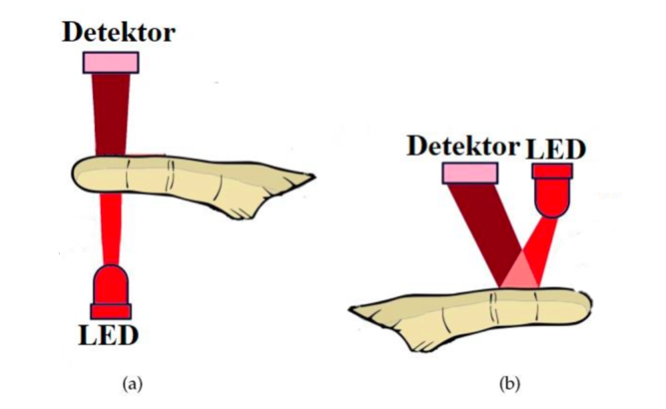
\includegraphics[width=0.8\textwidth]{./obrazky/snimaniPPG.png}
	\caption[Snímání PPG signálu]{Transmisní režim (a) a reflexní režim (b), upraveno z \cite{ENIKÖ}.}
	\label{fig:snimaniPPG}
\end{figure}

\acs{PPG} senzory jsou obvykle umístěny na prstech, uchu nebo na zápěstí, kde mohou efektivně monitorovat průtok krve.

V současné době se \acs{PPG} technologie neustále vyvíjí a rozšiřuje o nové aplikace.
Například, pokročilé algoritmy zpracování signálu a strojové učení otevírají cestu k přesnějšímu a spolehlivějšímu odhadu různých fyziologických parametrů.
Tato vylepšení mají potenciál výrazně zlepšit diagnostiku a monitorování zdravotního stavu v reálném čase.
To může vést ke kvalitnější prevenci a efektivnější léčbě mnoha kardiovaskulárních či respiračních onemocnění.

Tato technologie funguje na fyzikálním principu, při kterém okysličeným hemoglobinem prochází do fotoreceptoru jiná vlnová délka než odkysličeným hemoglobinem \cite{Orphanidou2018}.

% ----------------------------------------------------------------------- %
\section{\acs{PPG} signál}

Obrázek \ref{fig:signalPPG} nám ukazuje, že \acs{PPG} signál vykreslujeme na základě množství světla, které dopadlo na detektor a prošlo skrz tkáň, nebo se od ní odrazilo.
Signál se skládá ze dvou hlavních složek: pulzní (\acs{AC}) složky a ne-pulzní (\acs{DC}) složky.

Pulzní složka (\acs{AC}) \acs{PPG} signálu je synchronní se srdečními cykly a odráží změny objemu krve spojené s každým srdečním cyklem.
Tato složka je pro účel naší práce zásadní.
\acs{AC} složka je ovlivněna cyklickými změnami v objemu arteriální krve pod tlakem srdečních kontrakcí.

Na druhé straně ne-pulzní složka (\acs{DC}) představuje základní hodnotu absorpce světla tkání, která je ovlivněna různými faktory jako například barva kůže, složení tkáně a stabilní objem krve v místě umístěného senzoru.
Dále je ovlivněna vnějšími faktory, jako jsou specifikace měřicí technologie a podmínky okolního osvětlení \cite{ENIKÖ}\cite{Park2022}.

Počátek pulzu v \acs{PPG} signálu je obvykle pozorován v nejnižším bodě předcházejícím systolické fázi, což také odpovídá bodu minimálního objemu krve v tepnách.
Vrchol systolické fáze, představující maximální objem krve, je klíčovým bodem pro analýzu dynamiky průtoku krve.
Po systolickém vrcholu klesá \acs{PPG} signál do diastolické fáze, kde se objevuje výrazný rys známý jako "diastolický zářez".
Tento zářez, následovaný sekundárním vrcholem, indikuje obrácení tlakového gradientu, jak srdeční cyklus pokračuje do diastoly.

Tvar \acs{PPG} vlny se mění na základě vnějších podnětů, fyziologického stavu a složení těla \cite{Park2022}.

\begin{figure}[ht]
	\centering
	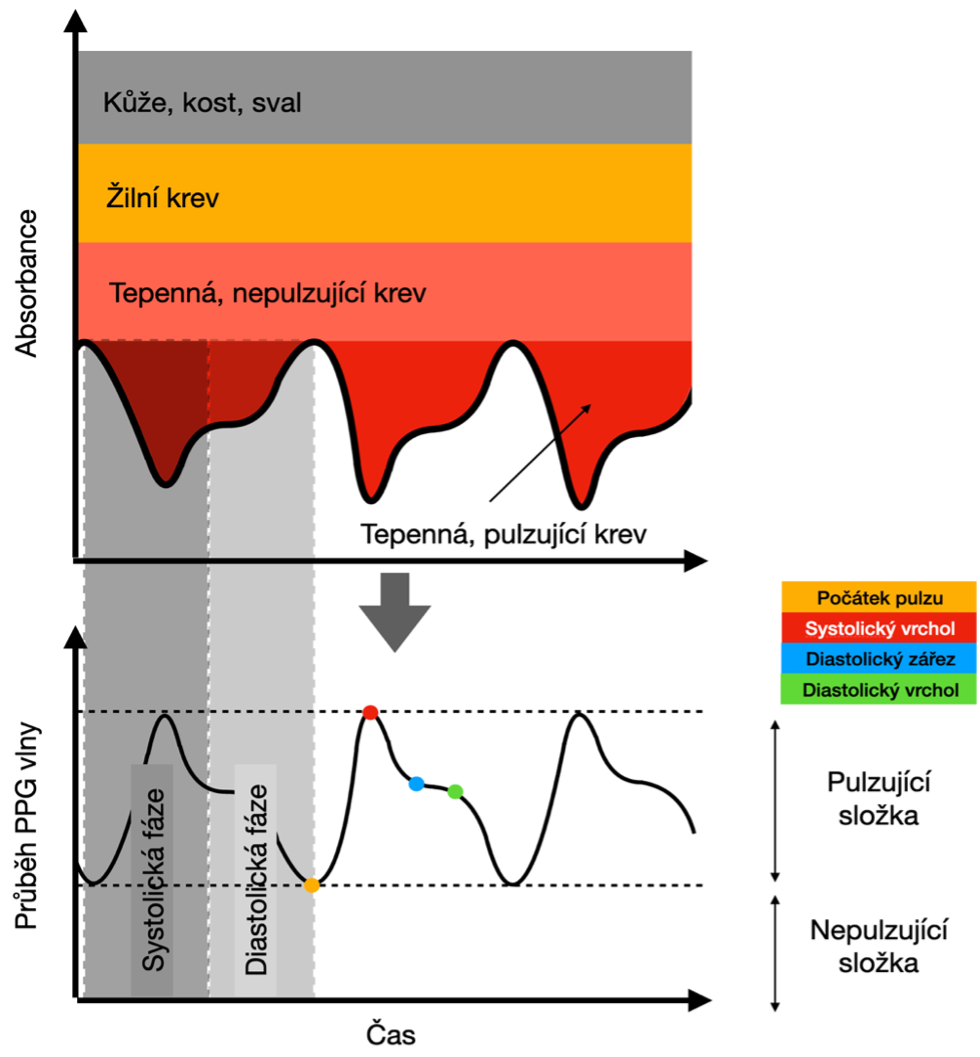
\includegraphics[width=0.8\textwidth]{./obrazky/signalPPG.png}
	\caption[Fiziologický popis PPG signálu]{Princip získání \acs{PPG} křivky a její popis, upraveno z \cite{Park2022}.}
	\label{fig:signalPPG}
\end{figure}
\raggedbottom
\chapter{Databáze}
\label{chap:databaze}

V této práci jsme využívali dvě databáze fotopletysmografických signálů: \textit{CapnoBase} a \textit{\acl{BUT PPG}}, pro kterou budeme v této práci používat zkrácený název \acs{BUT PPG}.

Na těchto databázích jsme testovali a porovnávali výsledky použitých algoritmů.
U databáze CapnoBase jsme porovnávali naměřené systolické vrcholy s referenčními hodnotami a díky tomu jsme porovnávali i rozdíl v srdeční tepové frekvenci (\acs{TF}).
U databáze \acs{BUT PPG} nebyly referenční hodnoty systolických vrcholů k dispozici, ale byly zde referenční hodnoty \acs{TF} signálů a ty jsme porovnávali s naměřenými výsledky.

\section{CapnoBase}
\label{sec:capnobase}

CapnoBase je veřejně dostupná databáze, která obsahuje osmiminutové záznamy od 42 dětských i dospělých pacientů, podstupujících plánované chirurgické zákroky včetně anestézie~\cite{CapnoBase}.

Součástí databáze jsou \acs{PPG}, \acs{EKG} a respirační signály, se vzorkovací frekvencí 300~Hz.
Pro každý záznam jsou navíc ručně označeny systolické vrcholy v \acs{PPG}, odvozené z \acs{EKG}, což umožňuje přesné ověření správnosti detekce tepů.
Autoři však nedoporučují databázi používat k trénování či dolaďování algoritmů~\cite{CapnoBase}.
Proto jsme ji použili pouze k testování použitých algoritmů a k porovnání výsledků s referenčními hodnotami.

Díky svým vlastnostem je CapnoBase vhodná k~posouzení robustnosti a přesnosti metod v~klinických situacích~\cite{Karlen2013, Charlton2022}.

\section{\acs{BUT PPG}}
\label{sec:but_ppg}

Databáze \acs{BUT PPG} vznikla na Fakultě elektrotechniky a komunikačních technologií \acs{VUT} za účelem zkoumání kvality \acs{PPG} záznamů a odhadu \acs{TF}.
V nové rozšířené verzi obsahuje 3,888 desetisekundových měření od 50 dobrovolníků (25 žen a 25 mužů) ve věku 19 až 76~let, a to v klidu i při různých typech pohybových aktivit.
Fotopletysmografické záznamy byly pořízeny chytrými telefony \textit{Xiaomi~Mi9} a \textit{Huawei~P20~Pro} se vzorkovací frekvencí 30~Hz.
Pro referenční \acs{EKG} a akcelerometrická (\acs{ACC}) data byl použit mobilní senzor \textit{Bittium Faros~360 (nebo 180)} se vzorkovacími frekvencemi 1,000~Hz pro \acs{EKG} a 100~Hz pro \acs{ACC}~\cite{BUT_PPG}.
Surový \acs{PPG} signál byl extrahován z červené složky nahraného videa (viz.~\ref{fig:videoZaznamPPG}).

Každý \acs{PPG} záznam byl synchronizován s \acs{EKG} a rozdělen do desetisekundových segmentů, které následně hodnotilo tři až pět expertů.
Pro označení kvality vycházeli výhradně z rozdílu mezi \acs{TF} odhadnutou z \acs{PPG} a referenční tepovou frekvencí z \acs{EKG}.
Pokud byla odchylka do pěti úderů za minutu, bylo dané měření označeno jako „dobré“ (1), jinak jako „špatné“ (0).
Tato hranice vychází z mezinárodní normy IEC 60601-2-27 a v databázi \acs{BUT PPG} je aplikována ještě přísněji~\cite{BUT_PPG}.

Přibližně polovina záznamů vznikla přiložením prstu na zadní kameru a LED, druhá pak snímáním ucha v poloze připomínající telefonování.
V novější části databáze se rozšiřuje množství subjektů i situací, včetně manipulací s osvětlením, vyšším tlakem prstu na čočku, mluvením či chůzí, a nově se přidávají i údaje o krevním tlaku, glykémii a saturaci krve kyslíkem.

Díky této variabilitě podmínek a bohatým anotacím je \acs{BUT PPG} unikátním zdrojem pro testování robustnosti algoritmů detekce \acs{TF} a pro posuzování použitelnosti krátkých \acs{PPG} signálů z mobilního telefonu v reálné praxi.

\begin{figure}[ht]
	\centering
	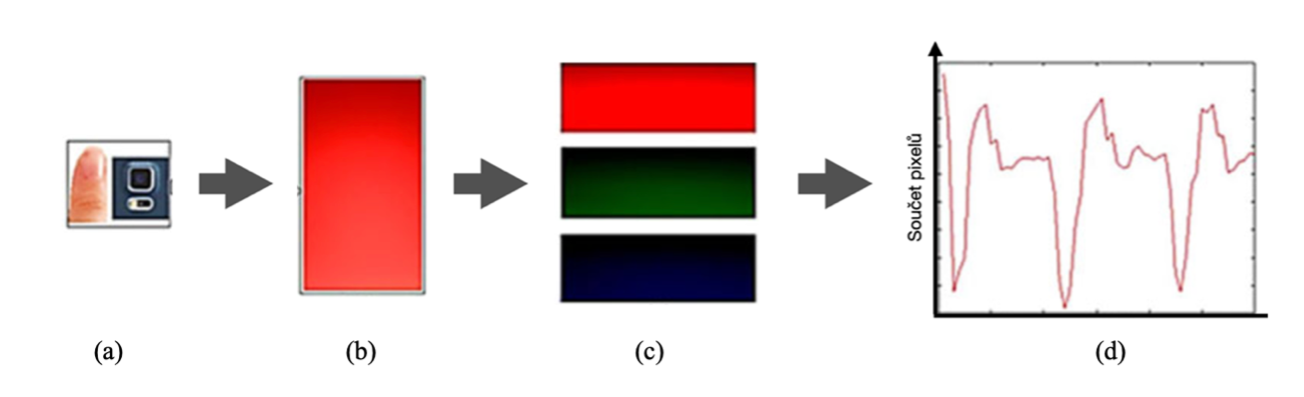
\includegraphics[width=0.8\textwidth]{./obrazky/videoZaznamPPG.png}
	\caption[Získání PPG signálu pro databázi \acs{BUT PPG}]{Záznam videa na kameru mobilního telefonu (a), jeden vybraný snímek ze záznamu (b), snímek rozložen na tři barevné složky (c), PPG signál vykreslený z červené složky (d), upraveno z~\cite{Siddiqui2016}.}
	\label{fig:videoZaznamPPG}
\end{figure}

Spojením klinicky orientované databáze CapnoBase a mobilně zaměřené \acs{BUT PPG} vzniká možnost vzájemného porovnání a ověření přesnosti algoritmů, které musejí obstát v rozdílných kontextech: v relativně stabilním, klinickém, prostředí a v krátkých záznamech z chytrého telefonu.

%%% PRAKTICKÁ ČÁST
\chapter{Elgendiho referenční algoritmus}
\label{chap:elgendi_neurokit}

Tato kapitola popisuje, jak lze ve fotopletysmografickém (\acs{PPG}) signálu nalézt systolické vrcholy s využitím Elgendiho algoritmu, který je implementován v~knihovně NeuroKit2.
NeuroKit2 reaguje na \uv{krizi reprodukovatelnosti} v psychologii a neurovědách a nabízí open-source kód, strukturovanou dokumentaci i podporu k začleňování funkcí přímo do výzkumných prací~\cite{NeuroKit2}.
Knihovna je dostupná na \url{https://github.com/neuropsychology/NeuroKit} (zdrojový kód) a \url{https://neurokit2.readthedocs.io/} (dokumentace) a její návrh umožňuje průběžný vývoj a modifikace.
V~kapitole~\ref{chap:PPG_teorie} byly již podrobně shrnuty principy \acs{PPG}, proto se zde zaměříme na samotnou detekci vrcholů a její realizaci.

\section{Obecná struktura algoritmu}
Algoritmus se skládá z několika kroků: \emph{filtrace} pomocí pásmové propusti, \emph{umocnění} signálu, vytvoření dvou \emph{klouzavých průměrů} a dvou \emph{prahů}, jak je zobrazeno na obrázku~\ref{fig:alg-scheme}~\cite{Elgendi2013}.
Vstupem je surový fotopletysmografický záznam, zatímco výstupem jsou konkrétní časové pozice nalezených systolických vrcholů.

\begin{figure}[htbp]
	\centering
	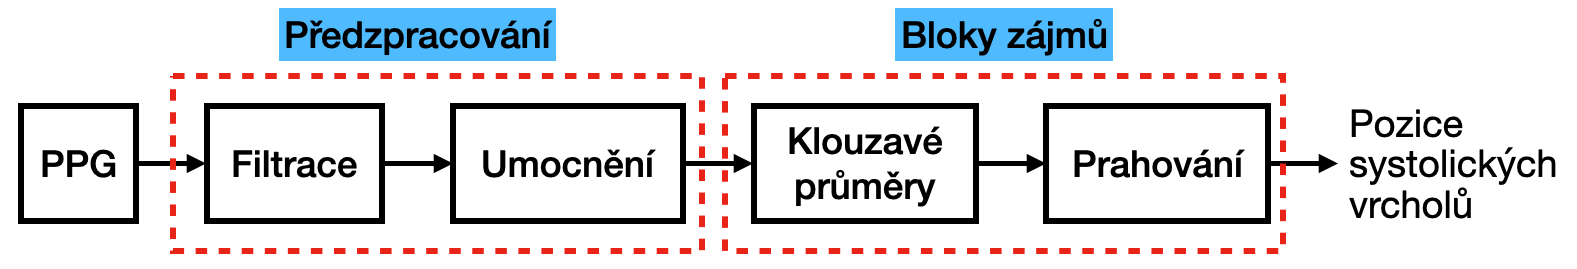
\includegraphics[width=1\textwidth]{./obrazky/ElgendiBlokSchema.png}
	\caption[Struktura Elgendiho algoritmu]{Zjednodušené schéma Elgendiho algoritmu~\cite{Elgendi2013}.}
	\label{fig:alg-scheme}
\end{figure}

\section{Předzpracování signálu}
Před samotnou detekcí je vhodné potlačit šum a odstranit pomalé změny amplitudy.
Elgendi~\cite{Elgendi2013} používá druhý řád Butterworthova filtru se zpracováním v~přímém i reverzním směru (tzv.~filtrace s nulovým fázovým posuvem).
Frekvenční charakteristika filtru byla nastavena na pásmo 0,5--8~Hz, což postačuje pro typické PPG kmitočty a dostatečně potlačí pásmový posun i vyšší frekvence nesouvisející se systolickými vrcholy.

Na obrázku~\ref{fig:filter-example} je ukázka amplitudové charakteristiky a zfiltrovaného úseku signálu.

\begin{figure}[htbp]
	\centering
	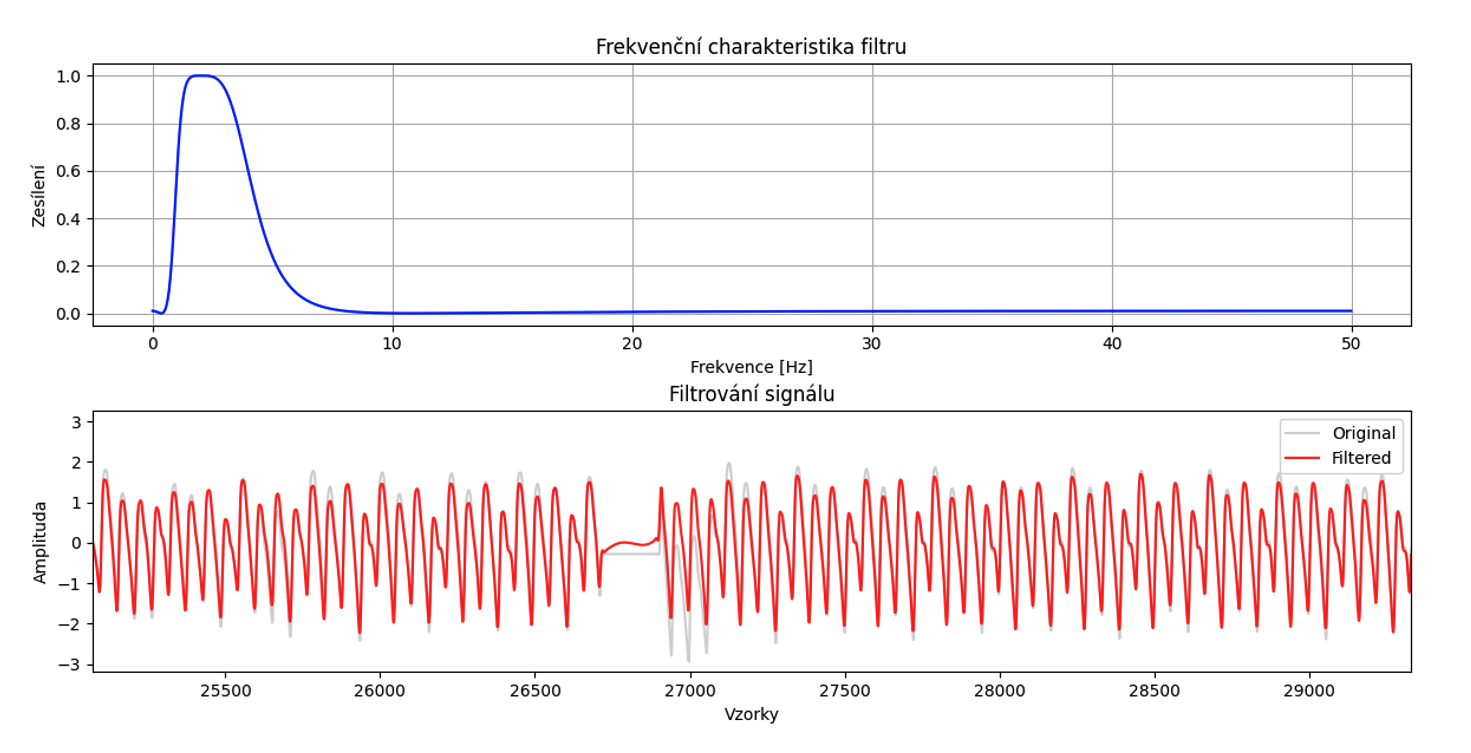
\includegraphics[width=0.8\textwidth]{./obrazky/ElgendiBandpass.png}
	\caption[Filtrace PPG signálu]{Horní graf: příklad amplitudové přenosové charakteristiky pásmové propusti. Dolní graf: znázornění filtrace PPG (šedě původní signál, červeně po filtraci).}
	\label{fig:filter-example}
\end{figure}

Po filtraci se signál umocňuje na druhou, aby se zdůraznily rozdíly mezi systolickou vlnou a ostatními složkami (například diastolickými zářezy).
Výsledná hodnota $y[n]$ po umocnění je:
\begin{equation}
	y[n] = Z[n]^2,
	\label{eq:square}
\end{equation}
kde $Z[n]$ je již vyfiltrovaný signál.
V~důsledku toho bývá systolický vrchol zdůrazněn na úkor diastolických zářezů nebo šumu~\cite{Elgendi2013}, jak je ilustrováno na obrázku~\ref{fig:squared-signal}.

\begin{figure}[htbp]
	\centering
	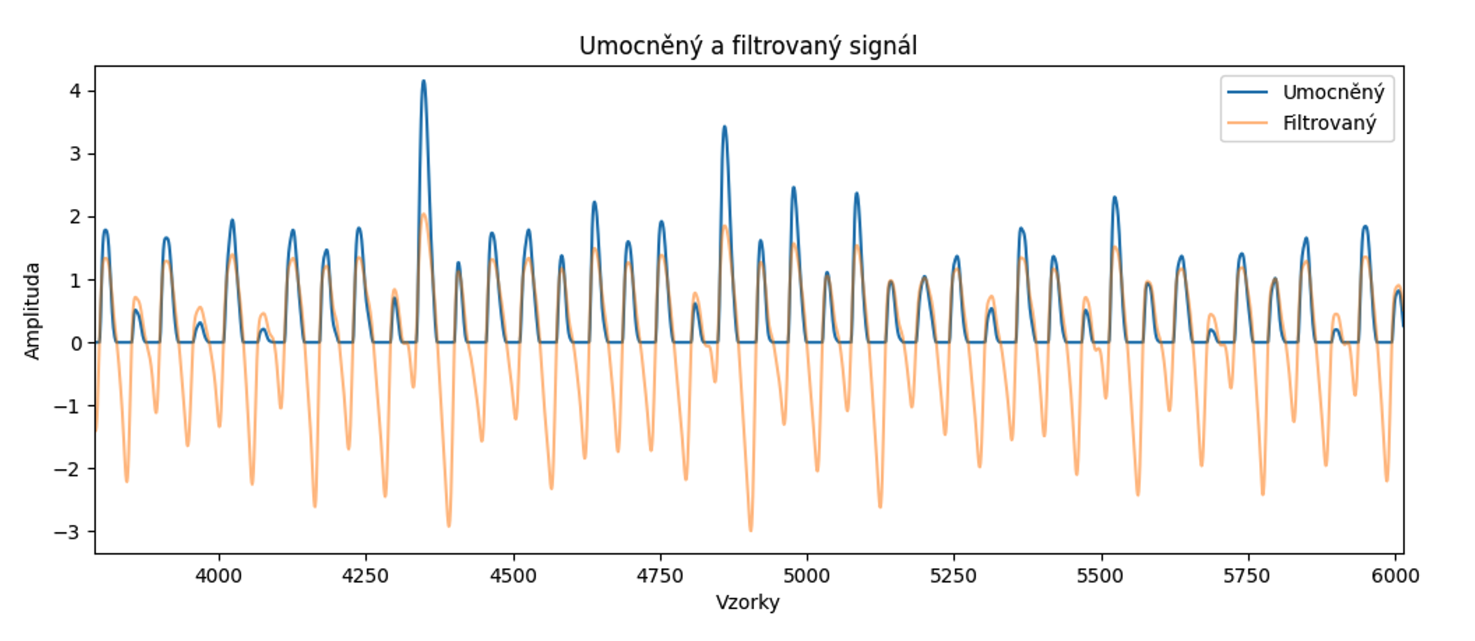
\includegraphics[width=0.8\textwidth]{./obrazky/ElgendiUpravenySignal.png}
	\caption[Umocněný a filtrovaný PPG]{Porovnání filtrovaného umocněného PPG.}
	\label{fig:squared-signal}
\end{figure}

\section{Dvoufázové prahování a nalezení vrcholů}
Po umocnění je potřeba určit, kde přesně hledat potenciální maximum, tedy systolický vrchol.
Pro tento účel využívá Elgendiho algoritmus dva různé klouzavé průměry~(\acs{MA}), které se liší délkou okna a následně dva prahy pro finální detekci vrcholů~\cite{Elgendi2013}.

% Krátké okno prvního klouzavého průměru přibližně odpovídá šířce systolické vlny, zatímco delší okno (druhého průměru) pokrývá délku celého srdečního cyklu.
% Na základě jejich rozdílu a adaptivních prahů se definují \uv{bloky zájmu}, kde by mohl ležet vrchol.
% V takto vymezeném úseku se hledá a bere maximální hodnota jako systolický vrchol.
% Souhrnně lze postup vyjádřit rovnicí

% Elgendiho algoritmus určuje systolické vrcholy dvoustupňovým postupem s~využitím dvou klouzavých průměrů a následného prahování~\cite{Elgendi2013}.
% Nejprve jsou zkonstruovány dva klouzavé průměry, které se liší délkou okna.
\acs{MA_P} zvýrazňuje oblast systolického vrcholu, zatímco \acs{MA_B} reprezentuje průměrnou úroveň v rámci celého tepu~\cite{Elgendi2013}.
Pomocí \acs{MA_B} se definuje první práh \acs{THR_1}, a to přičtením posuvného členu $\alpha$ k \acs{MA_B}, kde $\alpha$ je definována jako $\alpha = \beta\,\overline{z^2}$; v~této formuli je $\beta$ empirická konstanta (např.\ 0,02) a $\overline{z^2}$ střední hodnota umocněného a zfiltrovaného PPG signálu.
Porovnáním \acs{MA_P} s~\acs{THR_1} se identifikují tzv.\ bloky zájmu, které mohou obsahovat systolický vrchol či rušení.

V další fázi se tyto bloky podrobí druhému prahování, aby se odstranily ty, jejichž šířka je nižší, než se očekává pro systolickou vlnu~\cite{Elgendi2013}.
Pokud například platí $\mathrm{THR}_2 = W_1$, kde $W_1$ odpovídá délce systolického pulzu, pak všechny bloky užší než $\mathrm{THR}_2$ se považují za šum a odfiltrují se.
V akceptovaných blocích se následně najde nejvyšší hodnota signálu, která je interpretována jako poloha systolického vrcholu.
Tímto dvoustupňovým přístupem lze eliminovat falešné úseky způsobené diastolickou vlnou či jinými artefakty, a robustně tak určit polohu hlavního vrcholu~\cite{Elgendi2013}.

% \begin{figure}[htbp]
% 	\centering
% 	\includegraphics[width=0.78\textwidth]{blocks_detection.jpg}
% 	\caption[Oblasti hledání vrcholů]{Zobrazení umocněného signálu (tmavě modře), filtrovaného signálu (světle modře) a dvou klouzavých průměrů (zelené křivky). Šedé pruhy znázorňují vybrané úseky (bloky), kde hledáme maximum jako systolický vrchol (červené body).}

% 	\label{fig:block-detection}
% \end{figure}

% Aby se předešlo vícenásobné detekci blízko sebe, zavádí se také minimální vzdálenost mezi detekovanými vrcholy. Tato vzdálenost je obvykle nastavena podle reálné fyziologie, např. 200~ms při klidové tepové frekvenci.

% \section{Integrace do NeuroKit2}
% Popsaný postup je implementován v knihovně NeuroKit2 volbou \verb|method="elgendi"| při volání funkce \verb|ppg_process|:
% \begin{verbatim}
% import neurokit2 as nk

% signals, info = nk.ppg_process(
% 	ppg_signal, sampling_rate=fs,
% 	method="elgendi",
% 	method_quality="templatematch"
% )
% \end{verbatim}
% Výstup \verb|signals| typicky obsahuje sloupec s~pozicemi vrcholů a okamžitými hodnotami TF, zatímco \verb|info| nese další kontextové informace, například seznam indexů vrcholů či parametry filtrace.

% \section{Zhodnocení kvality signálu}
% Metoda \verb|templatematch| porovnává tvar každého detekovaného pulzu s~referenční šablonou a vyhodnocuje, do jaké míry odpovídá typické morfologii PPG. Takový přístup zjišťuje, zda je příslušný úsek skutečně “kvalitní” a nemá výrazné artefakty. Výsledkem může být číselné skóre kvality nebo binární označení (kvalitní / nekvalitní).

% \section{Závěr}
% Elgendiho algoritmus, s~částečnými modifikacemi v NeuroKit2, nabízí robustní a do značné míry automatizované řešení detekce systolických vrcholů v PPG. Díky adaptivním prahům a využití dvou klouzavých průměrů dokáže úspěšně potlačit různé formy šumu a spolehlivě najít systolický vrchol. K~praktickému použití navíc poslouží modul \emph{Template-Matching}, který vyhodnotí důvěryhodnost každého detekovaného pulzu.


\chapter{Vlastní algoritmy}
\chapter{Využití Hjorthových deskriptorů na odhad TF a kvality signálů}
\label{ch:hjorth}
% Důvody použití Hjorthových deskriptorů pro odhad TF.
% - Metoda nevyžaduje identifikaci systolických vrcholů.
% Argumentace robustností vůči šumu a periodicitou PPG signálu.
% Hjorthovy deskriptory se běžně používají v EEG (např. pro klasifikaci stavů), ale pro TF z PPG je to méně časté - a tedy inovativní.
V této kapitole je popsán alternativní přístup k odhadu srdeční tepové frekvence (\acs{TF}) z fotopletysmografického signálu (\acs{PPG}), využívající Hjorthovy deskriptory.
Na rozdíl od standardních metod~\cite{ENIKÖ,Charlton2022,NeuroKit2}, které se opírají o detekci jednotlivých systolických vrcholů a výpočet \acs{IBI}, využívá tento přístup frekvenční vlastnosti analyzovaného signálu.
To je výhodou v případech, kdy je signál poškozen šumem, artefakty, nebo když je kladen důraz na výpočetní náročnost a rychlost algoritmu.

V podkapitole~\ref{sec:hjorth_kvalita} je popsán způsob využití Hjorthových deskriptorů pro odhad kvality signálu pomocí metody náhodného lesa (\acs{RF}).

Hjorthovy deskriptory představují trojici příznaků určených z časového průběhu signálu, původně zavedených Hjorthem v~roce 1970 pro kvantitativní popis elektroencefalografických (\acs{EEG}) signálů~\cite{Hjorth1970,Hjorth1973}.
Jedná se o \textit{aktivitu} (\(H_0\)), \textit{mobilitu} (\(H_1\)) a \textit{komplexitu} (\(H_2\)), které odrážejí střední výkon, střední úhlovou frekvenci a šířku pásma.
Jejich výpočet vychází čistě z časové domény a nevyžaduje Fourierovu transformaci.

V dostupné literatuře jsme nenašli studie, které by Hjorthovy deskriptory využívaly k odhadu \acs{TF} z \acs{PPG} signálu.
Proto v této práci navrhujeme a realizujeme nový přístup založený na Hjorthově mobilitě~(\(H_1\)).
Tu počítáme na filtrovaných a několikanásobně autokorelovaných signálech.
Struktura navrženého algoritmu je znázorněna na Obr.~\ref{fig:hjorth_schemata}.

\begin{figure}[h]
	\centering
	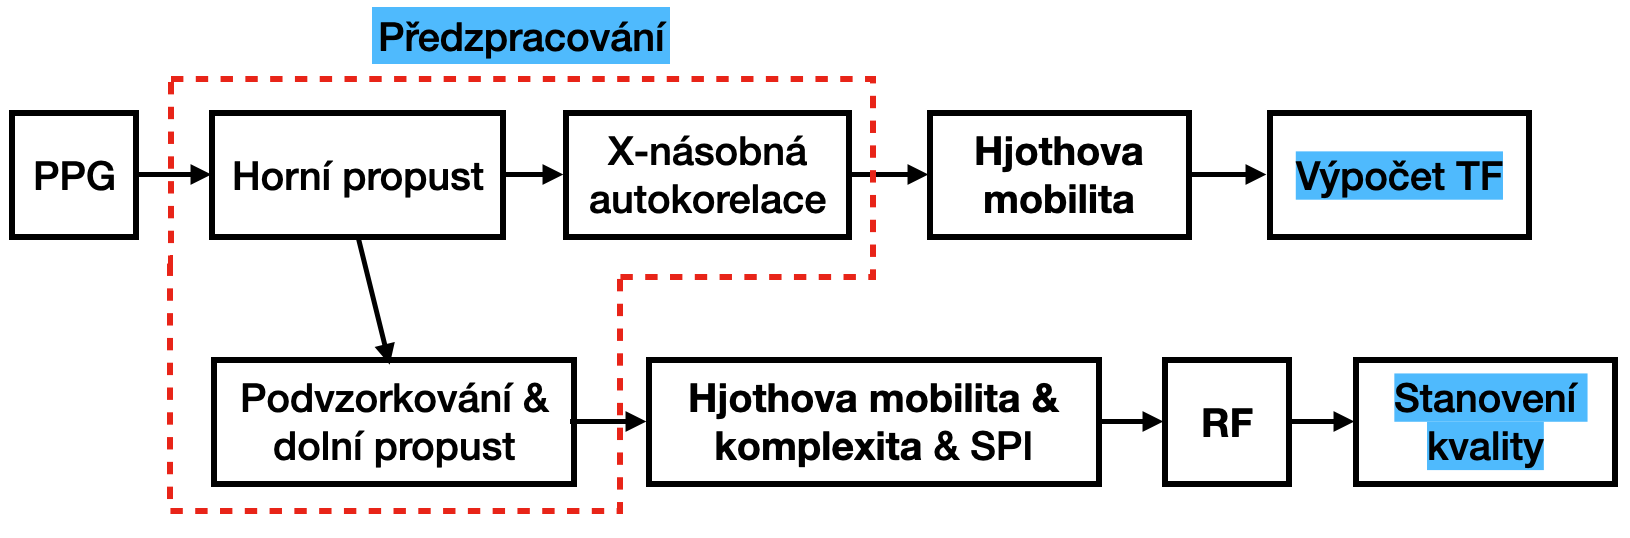
\includegraphics[width=1\textwidth]{./obrazky/hjorth_schema.png}
	\caption[Schéma našeho algorimu, který využívá Hjorthových deskriptorů]{Blokové schéma našeho využití Hjorthových deskriptorů.}
	\label{fig:hjorth_schemata}
\end{figure}

%%%%%%%%%%%%%%%%%%%%%%%%%%%%%%%%%%%%%%%%%%%%%%%%%%%%%%%%%%%%%%%%%%%%%%%%%%%%%%%%
%                                      TEP                                     %
%%%%%%%%%%%%%%%%%%%%%%%%%%%%%%%%%%%%%%%%%%%%%%%%%%%%%%%%%%%%%%%%%%%%%%%%%%%%%%%%
\section{Odhad TF pomocí Hjorthovy mobility}
\label{sec:hjorth_mobilita_tf}
% Načtení signálů z databází probíhá stejně jako u \ref{sec:alg_load}
% Rozdělení signálů je více modulativní, než u \ref{sec:alg_split} pro CapnoBase můžeme použít celý signál nebo libovolný počet oken s maximální délkou odpovídající 10s signálu. Pro BUT PPG (10s signály) to není možné.
Jak již bylo uvedeno, Hjorthova mobilita (\( H_1 \)) představuje odhad střední (resp. dominantní) frekvence signálu v časové oblasti, a to bez nutnosti výpočtu Fourierovy transformace.

Načtení signálů z databází probíhá stejným způsobem jako u našeho prvního algoritmu, popsaného v podkapitole~\ref{sec:alg_load}.
Odlišný přístup jsme však zvolili při dělení signálů.
Zatímco v předchozím algoritmu jsme signály z CapnoBase databáze dělili na minutové úseky, zde si můžeme ve vstupu funkce zvolit libovolný počet úseků, na které signál rozdělíme.
Maximální počet těchto úseků odpovídá situaci, kdy jeden úsek trvá 10~s.
Pokud zbyde po rozdělení signálu část, která je kratší než délka jednoho úseku, tak ji dále nezpracováváme.
Je proto důležité zvolit takové dělení, které minimalizuje délku zahozených úseků.
Alternativou by bylo upravit algoritmus tak, aby zbylé části zpracoval samostatně, nebo je přičlenil k předchozímu úseku.
Tím bychom však porovnávali signály různých délek, což by mohlo výsledky zkreslit.

\subsection*{Předzpracování}
\label{sec:predzpracovani}
% Odstranění stejnosměrné složky signálu -> standardizace signálu.
% High-pass filtraci pro odstranění respirační složky.
% Jak fungiuje vícenásobná autokorelace -> cílem je zvýraznění nejdominantnější periodickou složku.
% Grafy autokorelace, původní signál, frekvenční spektrum obou signálů.
% KEEP IN MIND: Nepotlačují se frekvence, ale složky o vyšších/nižších frekvencích.
U analyzovaných signálů jsme provedli standardizaci.
Nejprve jsme odstranili stejnosměrnou (\acs{DC}) složku signálu, tedy jeho střední hodnotu \(\mu\).
Tento krok slouží k centrování signálu kolem nuly, čímž omezíme vliv \acs{DC} složky na výpočet rozptylu signálu.
Ve druhém kroku standardizace jsme dělili signál zbavený hodnoty \(\mu\) jeho směrodatnou odchylkou \(\sigma\).
Rovnice pro standardizaci signálu je následující:
\begin{equation}
	\label{eq:standardizace}
	x[n] = \frac{x[n] - \mu}{\sigma}.
\end{equation}

Následně byl signál filtrován Butterworthovým hornopropustným filtrem čtvrtého řádu s mezní frekvencí 0,5~Hz v obou směrech.
Jeho amplitudová charakteristika i její druhá mocnina jsou zobrazeny na Obr.~\ref{fig:hjorth_filter}.
Cílem této filtrace bylo potlačení respirační složky, přičemž prahová frekvence byla zvolena na základě předpokládané minimální hodnoty \acs{TF}, jak je uvedeno v podkapitole~\ref{sec:STF}.

\begin{figure}[!th]
	\centering
	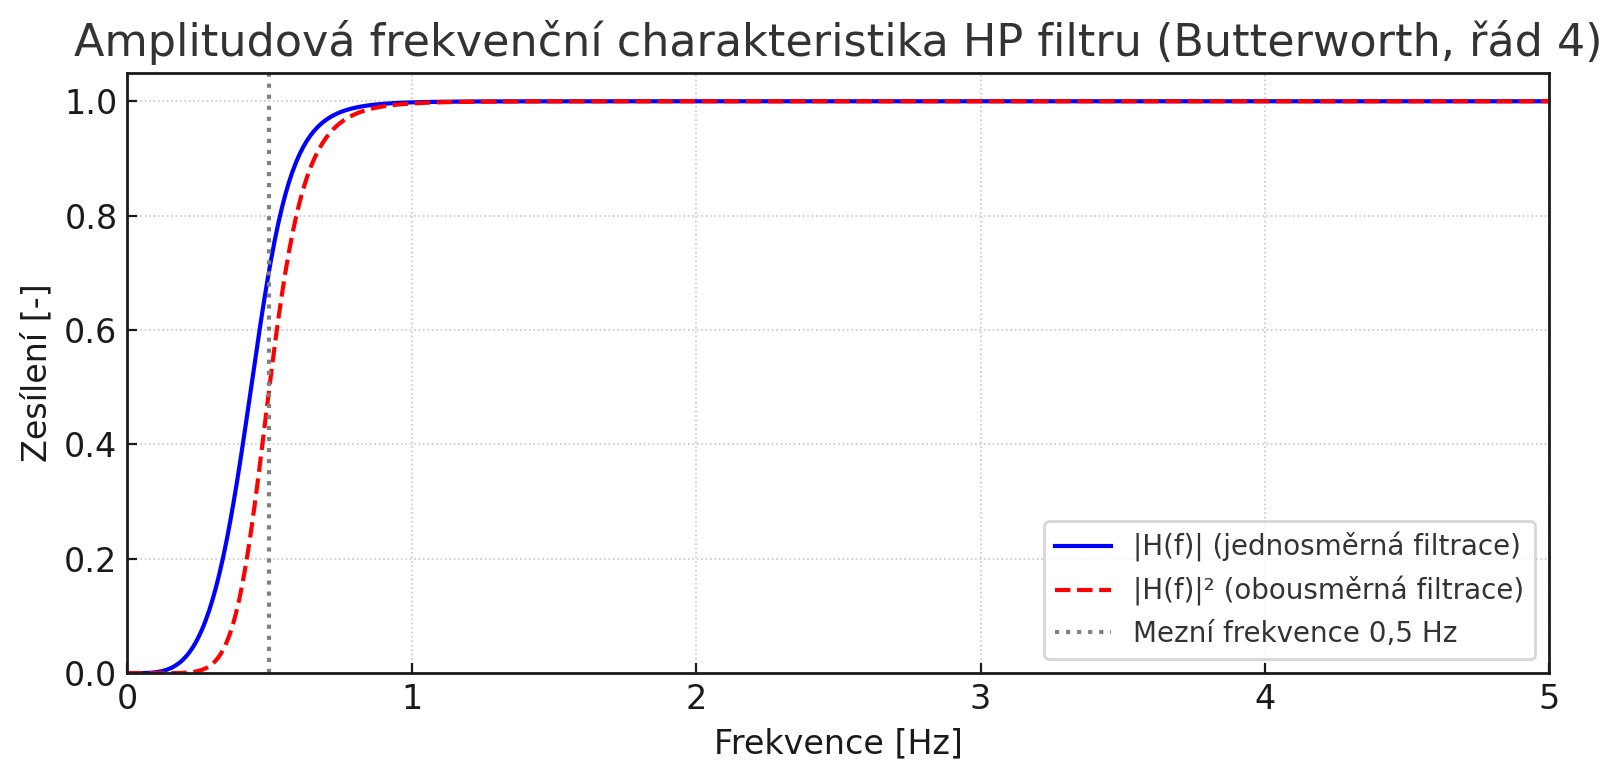
\includegraphics[width=1\textwidth]{./obrazky/hjorth/hp_filter_response_linear.png}
	\caption[Amplitudová charakteristika hornopropustného filtru]{Amplitudová charakteristika hornopropustného filtru.}
	\label{fig:hjorth_filter}
\end{figure}

Získaný signál byl dále sedmkrát za sebou autokorelován.
Autokorelace je operace, při které se signál koreluje sám se sebou při různých časových posunech.
Sedminásobná iterace byla zvolena na základě empirického pozorování výsledků na desetisekundových signálech z databáze CapnoBase.
Cílem opakované autokorelace je zvýraznění dominantní periodické složky signálu.
Klasická autokorelační funkce diskrétního signálu \( x[n] \) je definovaná jako:
\begin{equation}
	r_x[m] = \sum_{n=0}^{N-m-1} x[n] \cdot x[n+m],
\end{equation}
kde \( N \) je délka signálu a \( m \) je zpoždění.
Výpočet probíhal ve frekvenční oblasti pomocí rychlé Fourierovy transformace, čímž se snížila výpočetní náročnost na~\(O(i \cdot N \log N)\), kde~\(i\) je počet iterací autokorelace.
Bez použití \acs{FFT} by byla složitost \(O(N^2)\).

Po každé iteraci autokorelace byl signál převeden do rozsahu~\(<-1, 1>\) pomocí normalizace podle maximální absolutní hodnoty:
\begin{equation}
	\hat{x}[n] = \frac{x[n]}{\max |x[n]|}.
\end{equation}
Tato normalizace byla nezbytná, protože iterovaná autokorelace způsobuje exponenciální nárůst hodnot, což by vedlo k numerické nestabilitě a zkreslení výpočtu Hjorthových deskriptorů.

Opakovanou autokorelací dochází ke zvýšení spektrální ostrosti pro dominantní frekvenční složku, což jsme vyhodnotili jako žádoucí pro náš účel.

Porovnání spektra signálu před a po iterované autokorelaci je znázorněno na Obr.~\ref{fig:hjorth_predzpracovani}.
Horní část grafu zobrazuje časové průběhy původního, filtrovaného a autokorelovaného signálu, spodní část pak odpovídající spektra získaná pomocí rychlé Fourierovy transformace.
Amplitudové spektrum bylo vypočteno výhradně pro účely vizualizace a nefiguruje v samotném výpočtu Hjorthových deskriptorů.
Pro účely porovnání byla všechna spektra převedena na relativní jednotky pomocí normalizace vůči maximální hodnotě amplitudy daného signálu.

\paragraph{}
U běžných \acs{PPG} signálu odpovídají periodické složky systolickým fázím, diastolickým fázím a respiračním složkám.
Pro potlačení respiračních složek jsme použili hornopropustný filtr a pro potlačení složek diastolických fází jsme použili sedm iterací autokorelace.

\begin{figure}[!th]
	\centering
	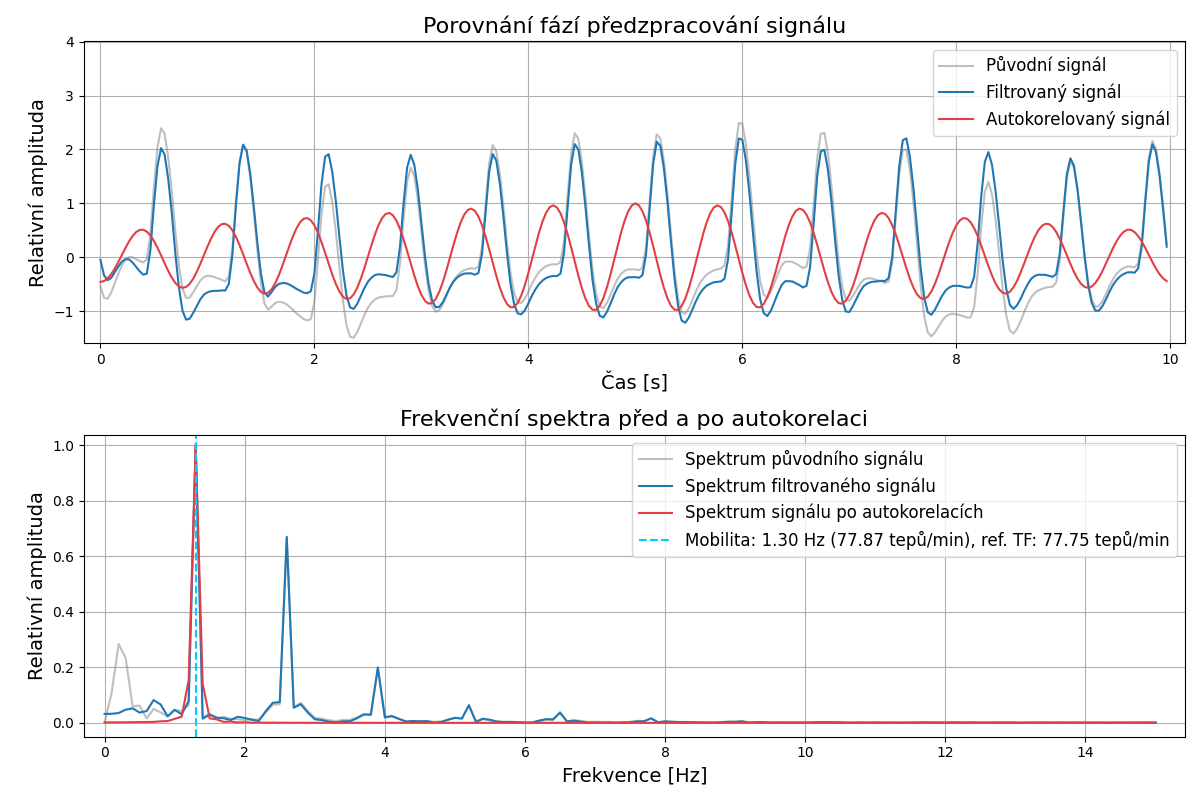
\includegraphics[width=1\textwidth]{./obrazky/hjorth_preprocess.png}
	\caption[Porovnání původního, filtrovaného a autokorelovaného signálu]{Porovnání původního, filtrovaného a autokorelovaného signálu.}
	\label{fig:hjorth_predzpracovani}
\end{figure}

\subsection*{Výpočet TF z mobility}
\label{sec:TF_mobilita}
% Vysvětlení co znamenajá mobilita a jak se počítá -> vzorec.
% Jak se počítá TF z mobility - vzorec.
% první diference = aproximujeme dva body vedle sebe
Po předzpracování signálu jsme vypočítali Hjorthovu mobilitu.
Ta je definována~\cite{Hjorth1970,Geetika2022} jako druhá odmocnina poměru rozptylu první derivace signálu ku rozptylu signálu samotného:
\begin{equation}
	\label{eq:hjorth_mobility}
	H_1 = \sqrt{ \frac{ \mathrm{var}(x[n] - x[n-1]) }{ \mathrm{var}(x[n]) } }
	= \sqrt{ \frac{ \mathrm{var}(x') }{ \mathrm{var}(x) } }
	= \frac{ \sigma_{x'} }{ \sigma_{x} }.
\end{equation}
Jelikož pracujeme v diskrétním prostředí, je derivace aproximována první diferencí.

Rozptyl signálu \( x \) je dán vztahem:
\begin{equation}
	\label{eq:hjorth_var_signal}
	\mathrm{var}(x) = \frac{1}{N} \sum_{n=0}^{N-1} (x[n] - \mu)^2,
\end{equation}
kde \( N \) je délka okna a \( \mu \) je střední hodnota signálu.

Podobně je definován i rozptyl první derivace signálu \( x' \), přičemž první diferenci nelze definovat pro vzorek \( n = 0 \), takže součet začíná až od \( n = 1 \):
\begin{equation}
	\label{eq:hjorth_var_signal_diff}
	\mathrm{var}(x') = \frac{1}{N - 1} \sum_{n=1}^{N-1} (x'[n] - \mu')^2.
\end{equation}

Z hodnoty \( H_1 \) jsme následně odvodili dominantní frekvenci \( f_{dom} \)~[Hz], kterou jsme vynásobili šedesáti, abychom dostali odpovídající hodnotu \acs{TF} v tepech za minutu:
\begin{equation}
	\const{TF}_{\textind{Hjorth}} = 60 \cdot f_{\textind{dom}} = \frac{60 \cdot H_{\textind{1}}}{2\pi}.
\end{equation}
Hodnota dominantní frekvence je graficky znázorněna i písemně zmíněna na Obr.~\ref{fig:hjorth_predzpracovani} společně s odpovídající tepovou frekvencí a referenční hodnotou \acs{TF} z databáze.

\paragraph{}
Přestože mají klasické metody detekce vrcholů~\cite{Elgendi2013} lineární průchod signálem s asymptotickou složitostí \( O(N) \), jejich praktická složitost může být vyšší kvůli víceprůchodovým algoritmům, adaptivním prahům, filtrováním nebo nastavováním bloků zájmu (popsané v podkapitole~\ref{sec:blocks}).

Naopak výpočet Hjorthovy mobility má sice po \( i \) iteracích autokorelace (prováděné pomocí \acs{FFT}) složitost \( O(i \cdot N \log N) \), avšak díky své jednoduchosti a absenci větvení může být v praxi rychlejší.

Výsledky odhadu \acs{TF} na základě Hjorthovy mobility jsou popsány v kapitole~\ref{ch:vysledky}, přičemž porovnání rychlosti exekuce algoritmů je uvedeno v~Tab.~\ref{tab:capnobase_comparison} a Tab.~\ref{tab:but_ppg_comparison}.

%%%%%%%%%%%%%%%%%%%%%%%%%%%%%%%%%%%%%%%%%%%%%%%%%%%%%%%%%%%%%%%%%%%%%%%%%%%%%%%%
%                                    KVALITA                                   %
%%%%%%%%%%%%%%%%%%%%%%%%%%%%%%%%%%%%%%%%%%%%%%%%%%%%%%%%%%%%%%%%%%%%%%%%%%%%%%%%
\section{Hodnocení kvality PPG signálů}
\label{sec:hjorth_kvalita}
% Vysvětlení co znamenajá mobilita a komplexita a jak se počítají -> vzorec.
% - Mobilita_filtr a Komplexita_filtr
% Vysvětlit jak se počítá SPI
% Jaké prahy jsme nastavili pro hodnocení kvality signálu.
Tato podkapitola popisuje metodu automatického hodnocení kvality \acs{PPG} signálů pomocí Hjorthových deskriptorů s využitím klasifikátoru typu náhodný les (\acs{RF}).
Cílem této analýzy je ověřit, zda kombinace indexu spektrální čistoty (\acs{SPI}) a Shannonovy entropie, postačuje k automatické binární klasifikaci \acs{PPG} signálů na základě jejich kvality definované referenčním algoritmem od Orphanidou z knihovny NeuroKit2~\cite{NeuroKit2}.

\subsection*{Segmentace a předzpracování signálů}
\label{subsec:segmentace_predzpracovani}
% KEEP IN MIND: Nepotlačují se frekvence, ale složky o vyšších/nižších frekvencích.
Klasifikátor byl trénován na signálech ze dvou databází: CapnoBase a \acs{BUT PPG}, jejichž záznamy se liší délkou, jak podrobněji popisujeme v kapitole~\ref{chap:databaze}.

Pro zajištění srovnatelnosti Hjorthových deskriptorů mezi oběma databázemi byly signály z CapnoBase rozděleny na nepřekrývající se segmenty o délce 10~s, což odpovídá délce jednotlivých záznamů v databázi \acs{BUT PPG}.
Tato segmentace zároveň přispívá ke konzistenci vstupních dat a zvyšuje přesnost rozhodování jednotlivých stromů klasifikátoru.

Následně byly signály z CapnoBase převzorkovány na vzorkovací frekvenci 30~Hz, aby odpovídaly frekvenci signálů z databáze \acs{BUT PPG}.
Převzorkování bylo realizováno pomocí funkce \texttt{resample} z knihovny \texttt{scipy}, která implementuje Fourierovu interpolaci.
Jelikož tato metoda neobsahuje předběžnou dolnofrekvenční filtraci, mohlo by při přítomnosti vyšších frekvenčních složek dojít k aliasingu.

Abychom tomuto jevu předešli, aplikovali jsme před převzorkováním dolnopropustný filtr typu Butterworth čtvrtého řádu s mezní frekvencí 14~Hz.
Tím jsme potlačili složky nad polovinou cílové vzorkovací frekvence a zachovali pouze spektrum relevantní pro analýzu srdeční činnosti.

Po sjednocení délky a vzorkovací frekvence byly všechny signály standardizovány~(\ref{eq:standardizace}).
V souladu s postupem uvedeným v podkapitole~\ref{sec:hjorth_mobilita_tf} jsme dále odstranili nízkofrekvenční složky pod 0,5~Hz.
Zde jsme navíc potlačili i složky nad 3,35~Hz (201~tepům za minutu), čímž jsme omezili spektrum pouze na fyziologicky očekávané rozsahy srdeční frekvence.

\subsection*{Výpočet příznaků pro náhodný les}
\label{subsec:rf_features}
% popsat komplexitu a z ní SPI
% komplexita definovaná v Hjorth1970 je ve VUT pojmenována jako "Relativní složitost"
Prvním příznakem je index spektrální čistoty (\acs{SPI}), který je definován jako převrácená hodnota komplexity:
\begin{equation}
	\label{eq:hjorth_SPI}
	SPI = \frac{1}{H_2} = \frac{\sigma_{x'}^2}{\sigma_{x''} \cdot \sigma_{x}} \; [-].
\end{equation}

% komplexita a z ní SPI
Hjorthova komplexita (\acs{H_2}) kvantifikuje míru toho, jak se signál v čase odchyluje od harmonického průběhu.
Je definována jako poměr mobility~(\ref{eq:hjorth_mobility}) první derivace signálu ku mobilitě samotného signálu~\cite{Hjorth1970,Geetika2022}:
\begin{equation}
	\label{eq:hjorth_complexity}
	H_{2} = \sqrt{ \frac{H_1(x')}{H_1(x)} }
	= \sqrt{ \frac{ \text{var}(x'') / \text{var}(x') }{ \text{var}(x') / \text{var}(x) } }
	= \frac{ \sigma_{x''} \cdot \sigma_{x} }{ \sigma_{x'}^2 } \; [-],
\end{equation}
kde $x$, $x'$, $x''$ jsou signál, jeho první derivace a jeho druhá derivace.
$\sigma_x$ označuje směrodatnou odchylku.
Pro čistě harmonický signál, jako je sinusoida, by vycházelo $H_2 = 1$.
S rostoucím podílem vyšších frekvenčních složek se však signál stává proměnlivějším, a tím roste hodnota \( H_2 \).
To znamená, že \acs{SPI}, definovaná jako obrácená hodnota komplexity, bude klesat s rostoucí nepravidelností signálu.

% Shannonova entropie
Druhým příznakem je Shannonova entropie, která měří míru neuspořádanosti signálu na základě jeho rozdělení hodnot.
Jde o metriku založenou na teorii informace, jež vyjadřuje očekávané množství informace potřebné k~popisu jedné hodnoty ze signálu:
\begin{equation}
	\label{eq:shannon_entropy}
	S = - \sum_{i=1}^{N} p_i \cdot \log_2(p_i) \; [\text{bit}],
\end{equation}
kde $p_i$ je pravděpodobnost, že hodnota signálu spadá do $i$-tého intervalu histogramu a $N$ je celkový počet binů.

Pro výpočet histogramu byl signál nejprve normalizován do intervalu $< 0, 1 >$ a následně rozdělen do $N = 30$ stejně širokých binů.
Tento počet byl zvolen empiricky jako kompromis mezi rozlišením a stabilitou odhadu, při vědomí, že konstantní délka signálu je 10~s a vzorkovací frekvenci 30~Hz.

Shannonova entropie nabývá nízkých hodnot u pravidelných signálů s úzkým rozdělením (např. téměř periodická sinusoida),
zatímco chaotické nebo arteficiální signály, jejichž hodnoty se rozprostírají napříč celým intervalem, vykazují vyšší entropii.

% Standardizace na konci
Oba příznaky jsou standardizovány pomocí funkce \texttt{StandardScaler}, aby byl zajištěn jejich jednotný váhový vliv při klasifikaci.

\subsection*{Náhodný les}
\label{subsec:random_forest}
% Klasifikátor je Random Forest, který je vhodný pro zpracování malého počtu příznaků.
% příznak == feature
% paramtery = vstupy do RandomForestClassifier class-y
% Vysvětlit jak funguje Random Forest
% Stratifikace = zajištění stejného poměru tříd v trénovací a testovací sadě
% výsledky hodnotíme pomocí F1 skóre z Cross-Validation
Pro odhad kvality signálů jsme použili již zmíněný klasifikátor náhodný les (\acs{RF}), který tvoří sadu rozhodovacích stromů a kombinuje jejich výstupy hlasováním.
Na rozdíl od lineárních modelů dokáže zachytit i nelineární vztahy mezi příznaky.

% parametry a jejich optimalizace
Použili jsme implementaci \texttt{RandomForestClassifier} z knihovny \texttt{scikit-learn} s výchozími parametry: \texttt{n\_estimators} = 100 (počet stromů), \texttt{max\_depth} = 5 (maximální hloubka stromu) a \texttt{max\_features} = \texttt{sqrt} (pro každý uzel se testuje náhodně vybraná odmocnina z celkového počtu příznaků).
Optimalizace těchto parametrů byla provedena pomocí metody \texttt{GridSearchCV} ze~stejné knihovny, která systematicky vybírá nejlepší kombinace z~námi předdefinovaných hodnot parametrů.
Pro zajištění deterministického chování jsme parametr náhodné inicializace nastavili na hodnotu \texttt{random\_state = 42}.

% rozdělení dat
Rozdělení datasetu do trénovací a testovací množiny proběhlo v poměru 60~\% ku 40~\%, přičemž jsme použili stratifikaci, abychom zachovali poměr tříd (kvalitní/nekvalitní signály).
Jelikož datová sada vykazovala nevyváženost tříd, aktivovali jsme parametr \texttt{class\_weight='balanced'}, který upravuje váhy jednotlivých tříd podle jejich četnosti.
To zajišťuje, že model nebude preferovat většinovou třídu, ať už kvalitní nebo nekvalitní.

Jednou z výhod \acs{RF} je možnost kvantifikovat důležitost jednotlivých příznaků na základě jejich vlivu na rozhodování stromů, což přispívá k interpretovatelnosti modelu a transparentnosti výsledků, jak je zobrazeno na Obr.~\ref{fig:hjorth_feature_importance}.

\begin{figure}[ht]
	\centering
	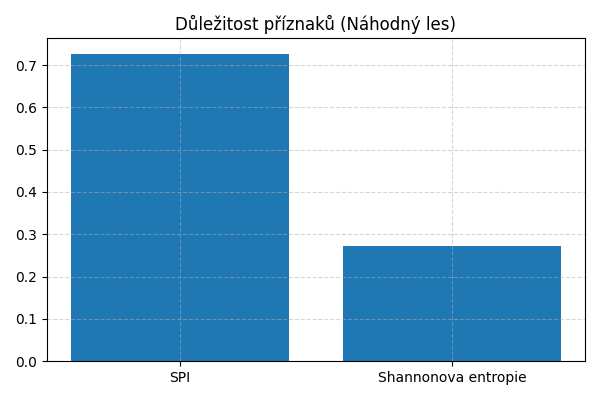
\includegraphics[width=0.8\textwidth]{./obrazky/quality/feature_importance.png}
	\caption[Důležitost příznaků pro klasifikaci kvality signálů pomocí náhodného lesa]{Důležitost příznaků pro klasifikaci kvality signálů pomocí náhodného lesa.}
	\label{fig:hjorth_feature_importance}
\end{figure}

% cross-validation
Výkonnost modelu jsme hodnotili pomocí pětinásobného křížového ověření, což umožňuje stabilní odhad generalizační chyby bez závislosti na konkrétním rozdělení dat.
Jako hlavní metriku jsme zvolili $F_1$ skóre, které je definované jako harmonický průměr mezi přesností (\acs{PPV}) a citlivostí (\acs{Se}).

Výstupem modelu je pravděpodobnostní binární skóre kvality signálů.
To lze chápat jako hlasování lesa o~každém testovaném signálu, zda je daný signál kvalitní nebo ne.

\subsection*{Referenční hodnota kvality}
\label{subsec:referencni_hodnota_kvality}
% nevěříme referenční hodnotě kvality z databáze BUT PPG
% Orphanidou et al. 2015 - adaptivní porovnávání tvaru pulzních vln
% NeuroKit2 - implementace
Databáze \acs{BUT PPG}~\cite{BUT_PPG,BUT_PPG_database} poskytuje binární anotace kvality signálů založené na schopnosti odhadnout tepovou frekvenci z~\acs{PPG}.
Segment je označen jako kvalitní, pokud alespoň tři z~pěti expertů určili \acs{TF} s~absolutní chybou do 5~tepů za minutu vůči referenci z~\acs{EKG}.
Tato anotace však vychází z~lidského úsudku a konkrétní implementace referenčního algoritmu, což omezuje její objektivitu a opakovatelnost.

Proto jsme se rozhodli použít alternativní metodu hodnocení kvality signálů založenou na práci Orphanidou et al.~\cite{Orphanidou2015} a její implementaci v knihovně \texttt{NeuroKit2}~\cite{NeuroKit2}.
Zvolený algoritmus posuzuje kvalitu signálu na základě tzv. adaptivního porovnávání tvaru pulzních vln.

V první fázi algoritmus aplikuje heuristická pravidla, která ověřují, zda se inter-beat intervaly a srdeční frekvence nachází ve~fyziologicky věrohodném rozmezí.
Pokud tyto pravidla nejsou splněny, je segment automaticky označen jako nekvalitní.
Ve druhé fázi se detekují jednotlivé pulzy v~signálu, vytvoří se průměrná šablona pulzní vlny a následně se spočítá korelační koeficient mezi touto šablonou a každým detekovaným pulzem.
Průměrná korelace slouží jako měřítko morfologické pravidelnosti a stability v~čase.

Výstupem je spojité skóre kvality pro každý pulz v rozsahu $<0,1>$, kde vyšší hodnoty značí vyšší míru podobnosti mezi pulzy.
Pro účely binární klasifikace jsme vypočítali průměrné skóre z výstupního řetězce hodnot a následně jsme zvolili prahovou hodnotu $0,9$, což odpovídá vysoké kvalitě signálu.
Tato metoda je plně automatická, replikovatelná a vhodná pro trénování algoritmů založených na strojovém učení.

Obr.~\ref{fig:orphanidou_mismatch} ukazuje rozptyl skóre kvality dle Orphanidou pro celou \acs{BUT PPG} databázi a jejich vztah k binární anotaci.
Je patrné, že se hodnoty kvalit neshodují.
Např. Obr.~\ref{fig:bad_quality_passed} zobrazuje jeden ze signálů, který byl experty označen jako kvalitní, ale hodnota kvality dle Orphanidou je přibližně 0,59.
Chyba referenčního odhadu \acs{TF} je u tohoto signálu 26~tepů za minutu.

Z těchto důvodů považujeme skóre podle Orphanidou za vhodnější základ pro trénink modelu automatického hodnocení kvality PPG signálu.

Úspěšnost algoritmů odhadující \acs{TF} budeme hodnotit pomocí obou referenčních hodnot kvality.
Výsledky těchto algoritmů budou popsány v kapitole~\ref{ch:vysledky}.

\begin{figure}[ht]
	\centering
	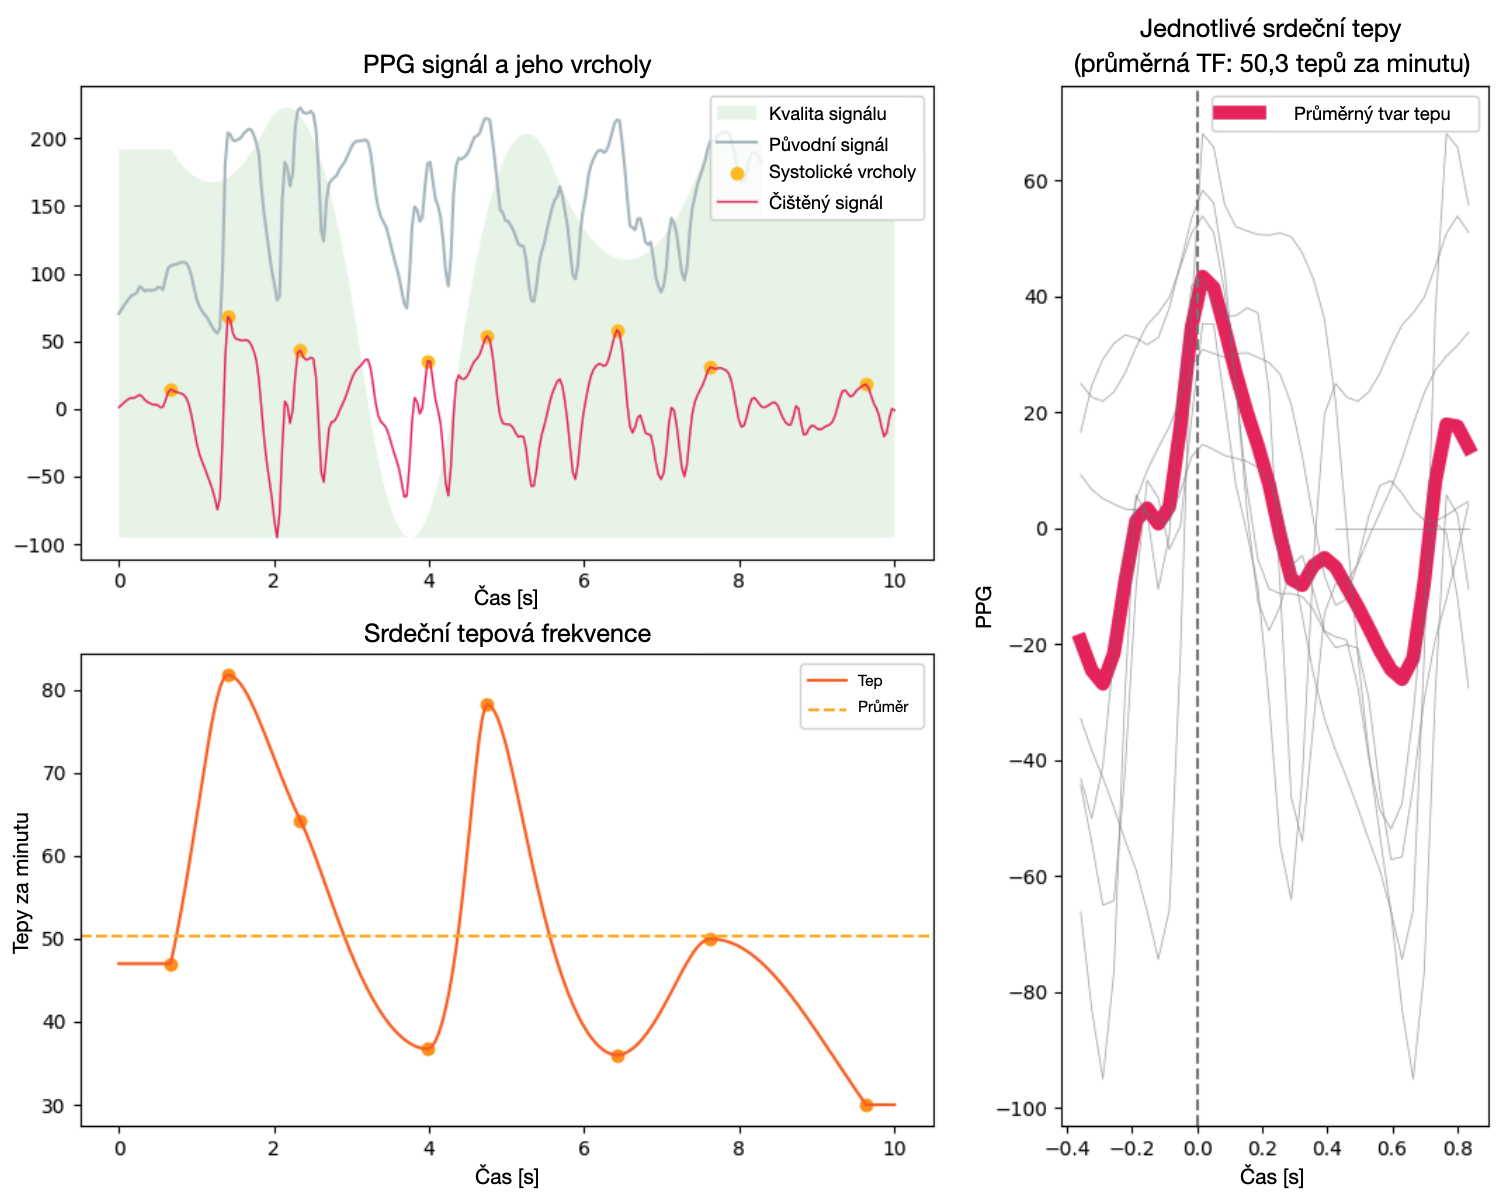
\includegraphics[width=1\textwidth]{./obrazky/quality/good_but_not_good.png}
	\caption[Signál označený databází za kvalitní]{Příklad signálu označeného jako kvalitní, přestože obsahuje silné artefakty a vykazuje vysokou chybu odhadu \acs{TF}.}
	\label{fig:bad_quality_passed}
\end{figure}

\begin{figure}[ht]
	\centering
	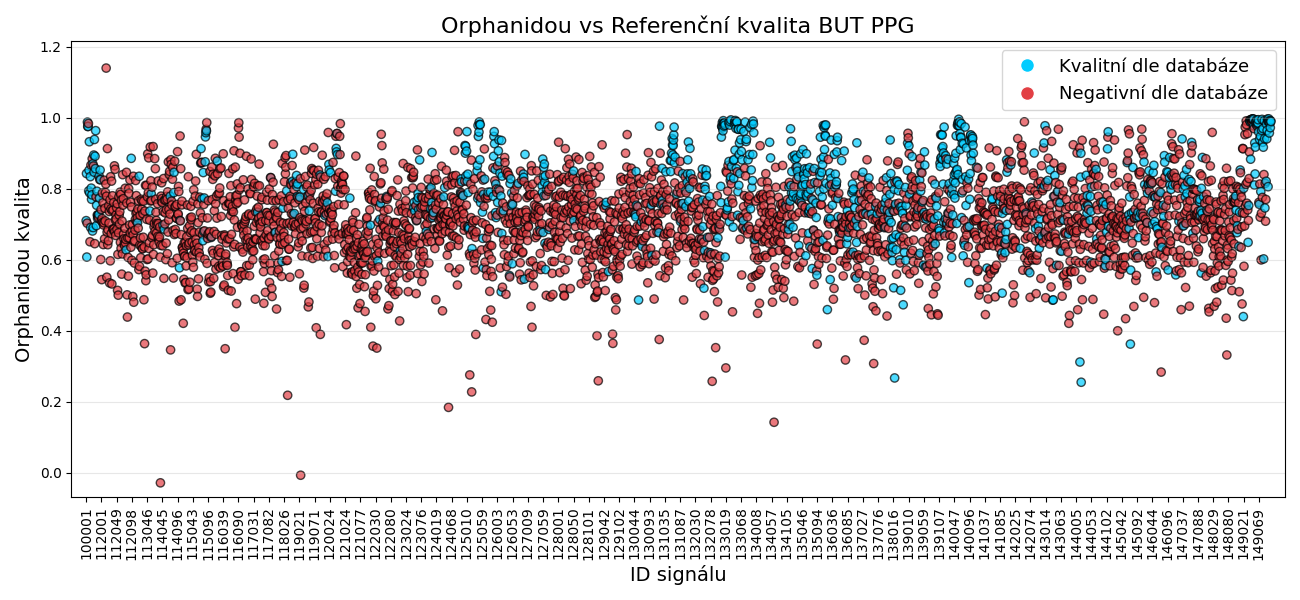
\includegraphics[width=1\textwidth]{./obrazky/quality/Orphanidou_Ref_Q.png}
	\caption[Porovnání kvality dle Orphanidou a referenční anotace z databáze \acs{BUT PPG}]{Porovnání kvality dle Orphanidou a referenční anotace z databáze \acs{BUT PPG}.}
	\label{fig:orphanidou_mismatch}
\end{figure}


%%% Vložení souboru 'text/vysledky' s popisem vysledků práce
% (rozdělte na více souborů či kapitol, pokud je vhodné)
\chapter{Výsledky} % Ukazujeme co jsme zjistili
\label{ch:vysledky}
% Čistě výstupy práce — tabulky, grafy, hodnoty, klasifikační skóre, výpočty, srovnání metod atd.
% Popis, co se naměřilo, vypočítalo, co model vrátil atd., bez hlubší interpretace.
Tato kapitola obsahuje výsledky odhadu tepové frekvence z fotopletysmografických signálů pomocí tří různých metod:
referenčního Elgendiho algoritmu, vlastního algoritmu založeného na detekci systolických vrcholů a nově navržené metody využívající Hjorthovy deskriptory.

Výsledky jsou vyhodnoceny samostatně pro obě použité databáze: CapnoBase a \acl{BUT PPG}.
Výsledky automatického posouzení kvality signálů jsou shrnuty v~podkapitole~\ref{sec:vysledky_kvalita}.

%%%%%%%%%%%%%%%%%%%%%%%%%%%%%%%%%%%%%%%%%%%%%%%%%%%%%%%%%%%%%%%%%%%
%                            CapnoBase                            %
%%%%%%%%%%%%%%%%%%%%%%%%%%%%%%%%%%%%%%%%%%%%%%%%%%%%%%%%%%%%%%%%%%%
\section{Výsledky pro databázi CapnoBase}
\label{sec:vysledky_capnobase}
% Popsat statistické metody, které jsme použili pro vyhodnocení kvality detekce vrcholů.
% Tabulka s metrikama
% Signál se pro tuto databázi nepodvzorkovává, ale máme původních 300 Hz.
% Fun fact = výsledky Hjortha je pro podvzorkované signály HORŠÍ
U této databáze máme k dispozici referenční hodnoty systolických vrcholů, a proto můžeme použít statistické metody pro vyhodnocení kvality detekce, jako je citlivost (\acs{Se}), pozitivní prediktivní hodnota (\acs{PPV}) a F1 skóre.
Citlivost vyjadřuje procento vrcholů, které použitý algoritmus správně rozpoznal z celkového počtu \textit{referenčních} vrcholů:
\begin{equation}
	\label{eq:se}
	\acs{Se} = \frac{\acs{TP}}{\acs{TP} + \acs{FN}} \cdot 100\%.
\end{equation}
Vyšší citlivost znamená nižší riziko, že algoritmus opomene detekovat skutečný vrchol.

Pozitivní prediktivní hodnota vyjadřuje procento vrcholů, které vybraný algoritmus určil správně z celkového počtu \textit{detekovaných} vrcholů:
\begin{equation}
	\label{eq:ppv}
	\acs{PPV} = \frac{\acs{TP}}{\acs{TP} + \acs{FP}} \cdot 100\%.
\end{equation}
Vyšší hodnota \acs{PPV} znamená, že algoritmus detekuje méně falešných vrcholů.

\acs{F1} skóre je harmonický průměr citlivosti a \acs{PPV} vyjádřen v procentech:
\begin{equation}
	\label{eq:f1}
	\acs{F1} = 2 \cdot \frac{Se \cdot PPV}{Se + PPV} \cdot 100\%.
\end{equation}

Tyto metriky počítáme pouze pro Elgendiho algoritmus a vlastní algoritmus detekce vrcholů, kvůli povaze algoritmu využívajícího Hjorthovu mobilitu, který neprovádí detekci vrcholů, ale přímo odhaduje tepovou frekvenci.
Když jsme je ale počítali, nastavili jsme toleranční pásmo pro výpočet matice záměn na $\pm$0,1~\acs{s}, které nám definuje, jak daleko od referenčního vrcholu se může detekovaný vrchol nacházet, aby byl považován za správně detekovaný.
V~Tab.~\ref{tab:capnobase_comparison} jsou hodnoty \acs{Se} a \acs{PPV} vypočítány ze součtu všech \acs{TP}, \acs{FP} a \acs{FN}.
\acs{F1} skóre je pak vypočítáno z těchto hodnot.

Dále jsme vyhodnotili průměrnou absolutní chybu (\acs{MAE}) mezi referenční a odhadovanou tepovou frekvencí dle rovnice~(\ref{eq:mae}).

\begin{equation}
	\label{eq:mae}
	\acs{MAE} = \frac{1}{N} \sum_{i=1}^{N} |TF_{i,ref} - TF_{i,est}|
\end{equation}

Jako dodatečné kritérium jsme stanovili poměr mezi dobře a špatně odhadnutými signály.
Za dobře odhadnuté byly považovány signály s \acs{MAE} menší než 5~\acs{bpm}, což odpovídá prahové hodnotě dle mezinárodního standardu IEC~60601-2-27 a metodice databáze \acs{BUT PPG}~\cite{BUT_PPG}.
V tabuce používáme označení \uv{d:š} pro poměr \uv{dobře:špatně} odhadnutých signálů.
% Po vypočítání průměrné kvadratické chyby (\acs{RMSE})~(\ref{eq:rmse}) mezi referenční a odhadovanou \acs{TF} jsme nastavili prahovou hodnotu \acs{RMSE} na XX tepů za minutu.

Poslední sledovanou metrikou byla výpočetní náročnost jednotlivých algoritmů, vyjádřená jako celkový čas potřebný ke zpracování celé databáze CapnoBase.
Výpočty probíhaly na platformě Apple M1.
Hodnoty jsou orientační a slouží pouze k vzájemnému srovnání mezi algoritmy.
Vzhledem k rozdílným charakteristikám databází (odlišná vzorkovací frekvence, délka i počet signálů, datový formát) nejsou časy mezi CapnoBase a \acs{BUT PPG} přímo srovnatelné.

Metriky přesnosti pro všechny tři algoritmy jsou uvedeny v~Tab.~\ref{tab:capnobase_comparison}, a to vždy pro různé délky vstupního signálu.

% table with comparison of methods
\begin{table}[!ht]
	\centering
	\caption[Srovnání metod odhadu TF na databázi CapnoBase]{Srovnání metod odhadu TF.}
	\label{tab:capnobase_comparison}
	\resizebox{\textwidth}{!}{
		\begin{tabular}{|l|c|c|c|c|c|c|}
			\hline
			\textbf{                  } &  \textbf{Se}  &  \textbf{PPV} &  \textbf{F1}  &     \textbf{MAE}     & \textbf{Poměr} & \textbf{Čas} \\
			\textbf{Metoda} (délka [s]) & \textbf{[\%]} & \textbf{[\%]} & \textbf{[\%]} & \textbf{[\acs{bpm}]} & \textbf{[d:š]} & \textbf{[s]} \\
			\hline\hline
			Elgendi (480)        & 99,81 & 99,89 & 99,85 & 0,31 &   42:0   &  16,1 \\
			\hline
			Elgendi (62,5)       & 99,23 & 99,88 & 99,55 & 0,35 &   336:0  &  17,9 \\
			\hline
			Vlastní vrcholová    & 99,34 & 99,91 & 99,63 & 0,31 &   42:0   &  2,4  \\
			detekce (480)        &       &       &       &      &          &       \\
			\hline
			Vlastní vrcholová    & 98,49 & 99,91 & 99,20 & 0,37 &   336:0  &  2,7  \\
			detekce (62,5)       &       &       &       &      &          &       \\
			\hline
			Hjorth (480)         &  --   &  --   &  --   & 1,52 &   40:2   &  2,6  \\
			\hline
			Hjorth (60)          &  --   &  --   &  --   & 0,80 &   332:4  &  2,7  \\
			\hline
			Hjorth (10)          &  --   &  --   &  --   & 0,61 &  2015:1  &  14,5 \\
			\hline
		\end{tabular}
		}
\end{table}

Na Obr.~\ref{fig:capnobase_SePPV_1min} a~Obr.~\ref{fig:capnobase_SePPV_8min} je znázorněno srovnání citlivosti a~přesnosti mezi vlastní metodou detekce vrcholů a~referenční Elgendiho metodou.
První obrázek zobrazuje výsledky pro minutové úseky (přeněji 62,5~s), zatímco druhý shrnuje výstupy pro celé osmiminutové záznamy.
Nejnižší hodnotu citlivosti vykazuje náš algoritmus ve druhé minutě signálu 0115, což odpovídá případu zobrazenému na Obr.~\ref{fig:capnobase_our_err}.

\begin{figure}[!ht]
	\centering
	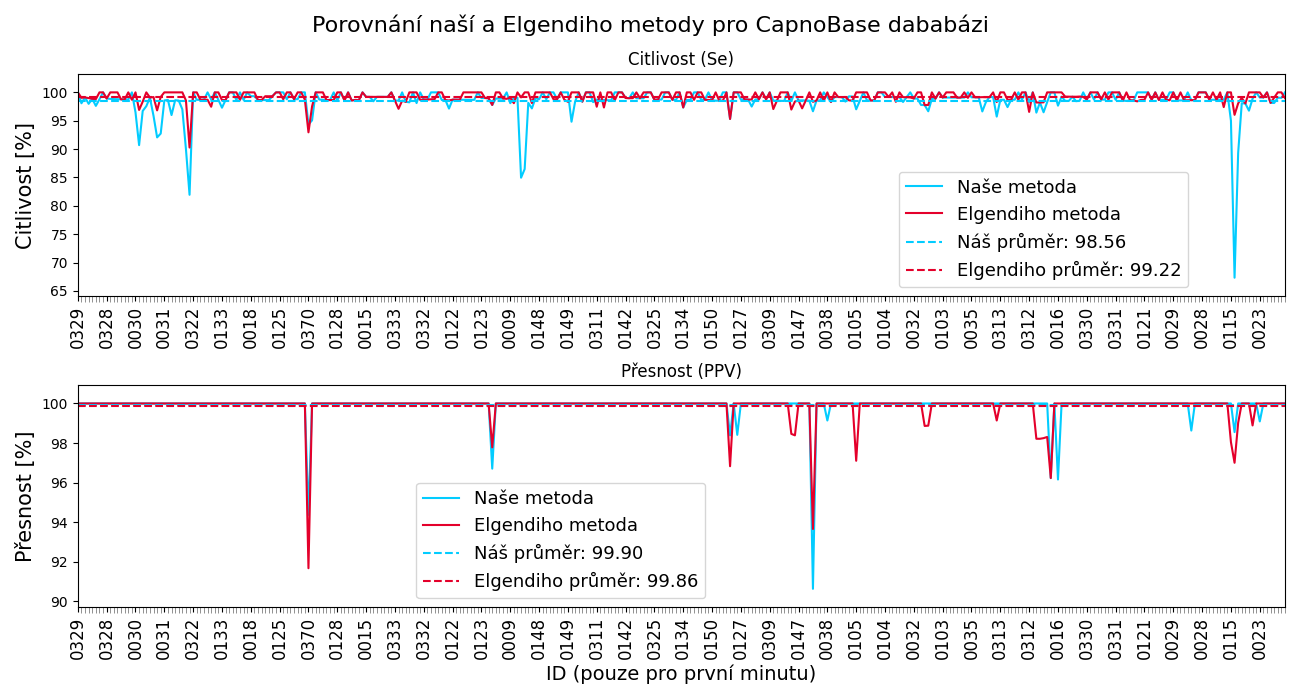
\includegraphics[width=1\textwidth]{./obrazky/vysledky/CB_Elgendi_Our_chunked.png}
	\caption[Srovnání metod detekující vrcholy pro minutové úseky]{Srovnání metod detekující vrcholy pro minutové úseky.}
	\label{fig:capnobase_SePPV_1min}
\end{figure}

\begin{figure}[!ht]
	\centering
	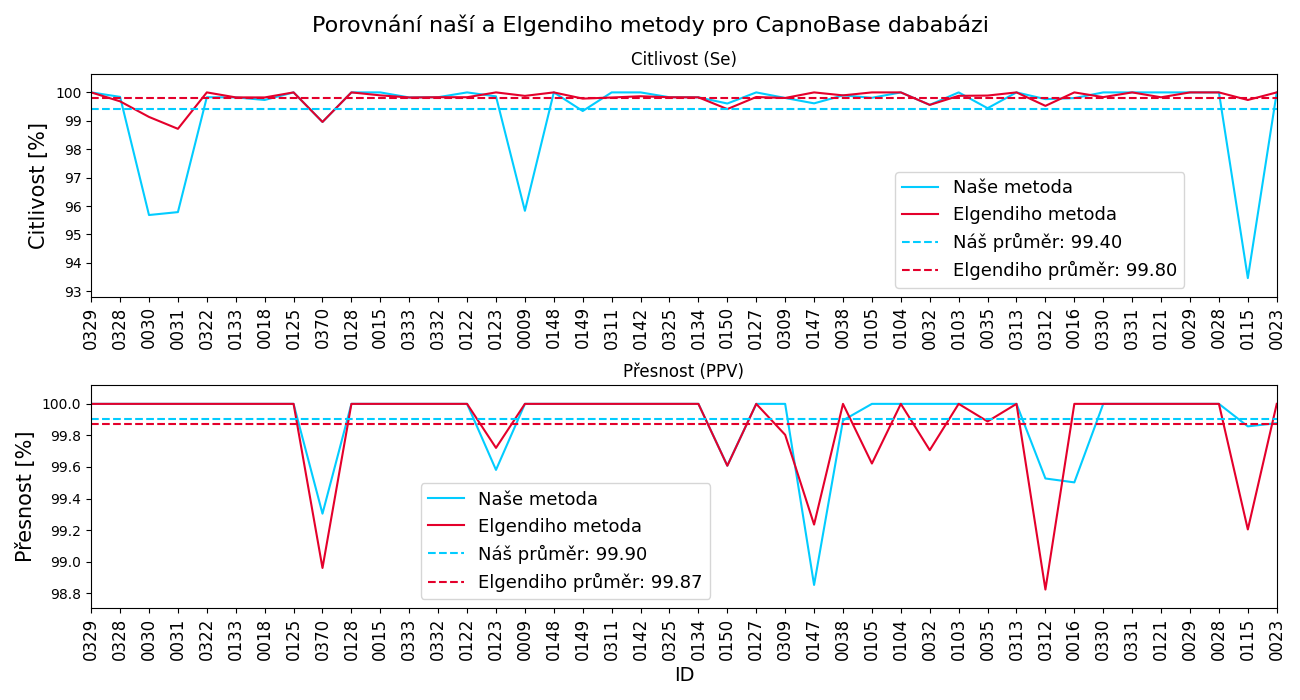
\includegraphics[width=1\textwidth]{./obrazky/vysledky/CB_Elgendi_Our_full.png}
	\caption[Srovnání metod detekující vrcholy pro celý signál]{Srovnání metod detekující vrcholy celý signál.}
	\label{fig:capnobase_SePPV_8min}
\end{figure}

\begin{figure}[!ht]
	\centering
	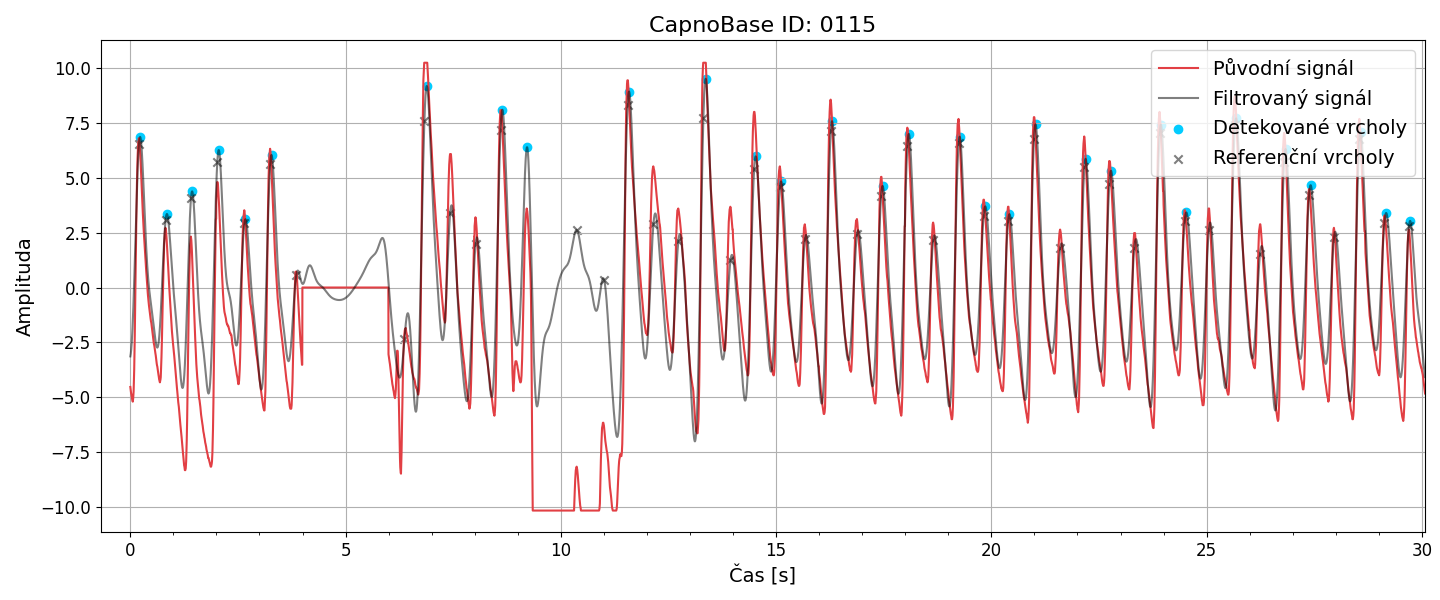
\includegraphics[width=0.9\textwidth]{./obrazky/vysledky/CB_Our_err.png}
	\caption[Chybný odhad \acs{TF} pomocí vlastní vrcholové detekce]{Chybný odhad TF pomocí vlastní vrcholové detekce.}
	\label{fig:capnobase_our_err}
\end{figure}

Je důležité poznamenat, že zobrazené hodnoty \acs{Se} a~\acs{PPV} se v~grafech liší od hodnot uvedených v~Tab.~\ref{tab:capnobase_comparison}.
V tabulce jsou hodnoty vypočteny jako agregovaná hodnota pro celou databází (tj. globální součet všech \acs{TP}, \acs{FP} a~\acs{FN})
Na druhou stranu, v~grafech jsou vypočítané hodnoty \acs{Se} a~\acs{PPV} individuálně a~z~těch je následně vypočítán a vykreslen průměr.
Tento přístup lépe odpovídá srovnání výkonnosti napříč jednotlivými záznamy, zatímco tabulková metrika lépe charakterizuje celkový výkon algoritmů.

Bland-Altmanovy grafy znázorněné na Obr.~\ref{fig:capnobase_BlandAltman_peaks} porovnávají rozdíl mezi odhadovanou a~referenční tepovou frekvencí pro obě metody detekce vrcholů.
Výsledky jsou rozděleny nejen podle použité metody (vlastní versus Elgendi), ale také podle délky analyzovaných úseků -- zvlášť pro celé osmiminutové signály a zvlášť pro jejich 62,5~s dlouhé úseky.
V grafech jsou vyznačeny průměrné odchylky (\acs{ME}) jako zelená přerušovaná čára, zatímco hranice shody, definované jako $\pm1,96 \cdot \acs{SD}$, jsou znázorněny červenými přerušovanými čarami.
Tato rozdílová analýza umožňuje posoudit, jak výrazně se odhady liší od referenčních hodnot a zda je chyba závislá na velikosti tepové frekvence.

\begin{figure}[!bh]
	\centering
	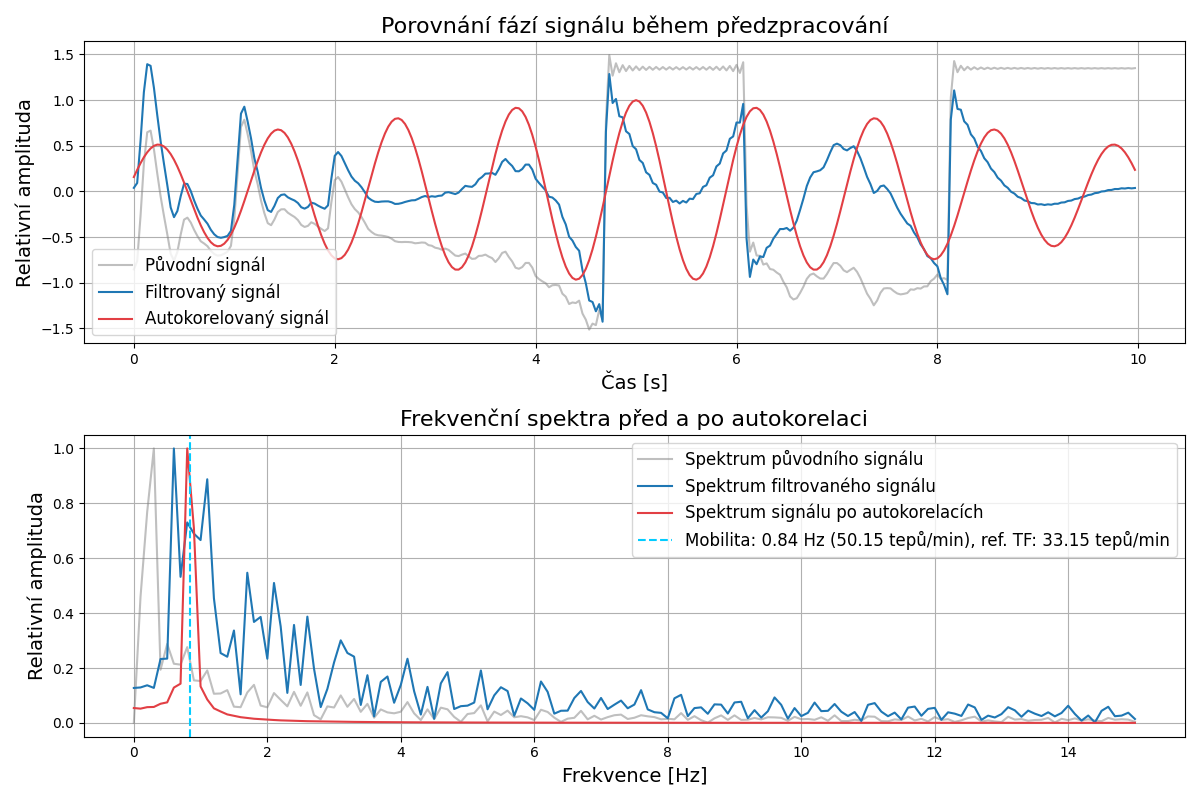
\includegraphics[width=0.9\textwidth]{./obrazky/vysledky/hjorth_preprocess_diffHR.png}
	\caption[Chybný odhad \acs{TF} pomocí Hjorthových deskriptorů u nekvalitního signálu]{Chybný odhad TF pomocí Hjorthových deskriptorů u nekvalitního signálu.}
	\label{fig:capnobase_hjorth_err}
\end{figure}

Obr.~\ref{fig:capnobase_BlandAltman_hjorth} zachycuje výsledky Bland-Altmanovy analýzy pro metodu využívající Hjorthovy deskriptory.
Grafy jsou opět rozděleny dle délky analyzovaných úseků: horní pro celé signály, prostřední pro minutové segmenty a spodní pro desetisekundové úseky.
V posledním grafu byly zahrnuty pouze signály označené jako kvalitní, čímž byl vyloučen jeden extrémně odlehlý případ (signál 0147, 25. minuta), který by vzhledem ke své vysoké chybě narušil škálu zobrazení.
Tento úsek je detailně zachycen na Obr.~\ref{fig:capnobase_hjorth_err}, kde je patrná výrazná deformace signálu a posun dominantní frekvence.
Společně s ním bylo vyloučeno dalších 15 signálů.

\begin{figure}[!ht]
	\centering
	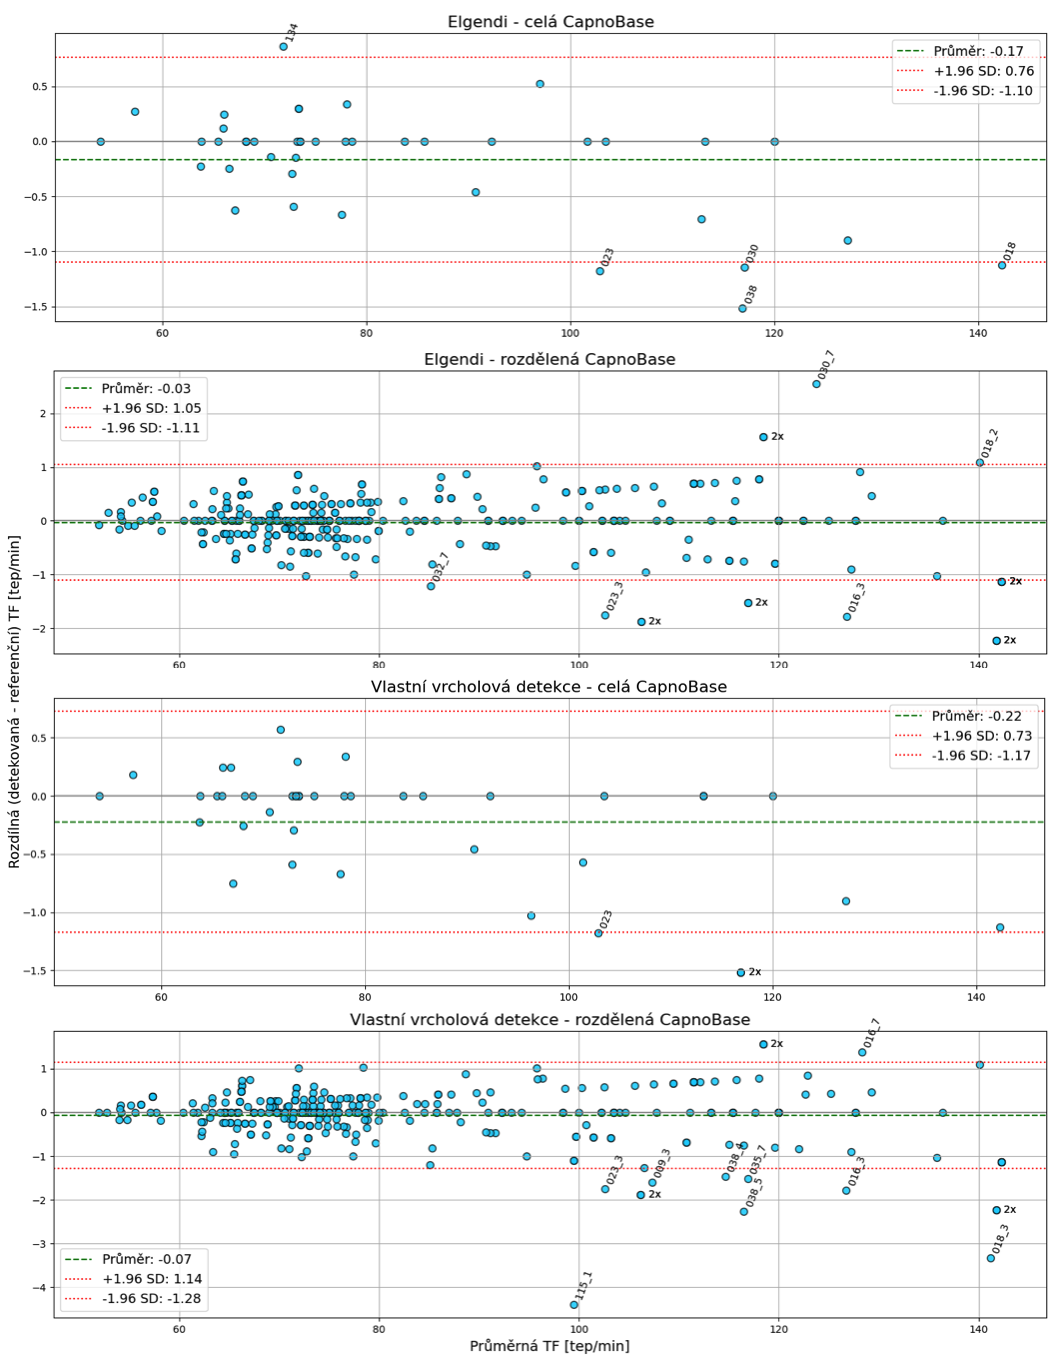
\includegraphics[width=1\textwidth]{./obrazky/vysledky/BlandAltman_CB_peaks.png}
	\caption[Bland-Altmanova analýza pro metody detekující vrcholy - CapnoBase]{Bland-Altmanova analýza pro metody detekující vrcholy.}
	% \vspace{-10mm}
	\label{fig:capnobase_BlandAltman_peaks}
\end{figure}

\begin{figure}[!ht]
	\centering
	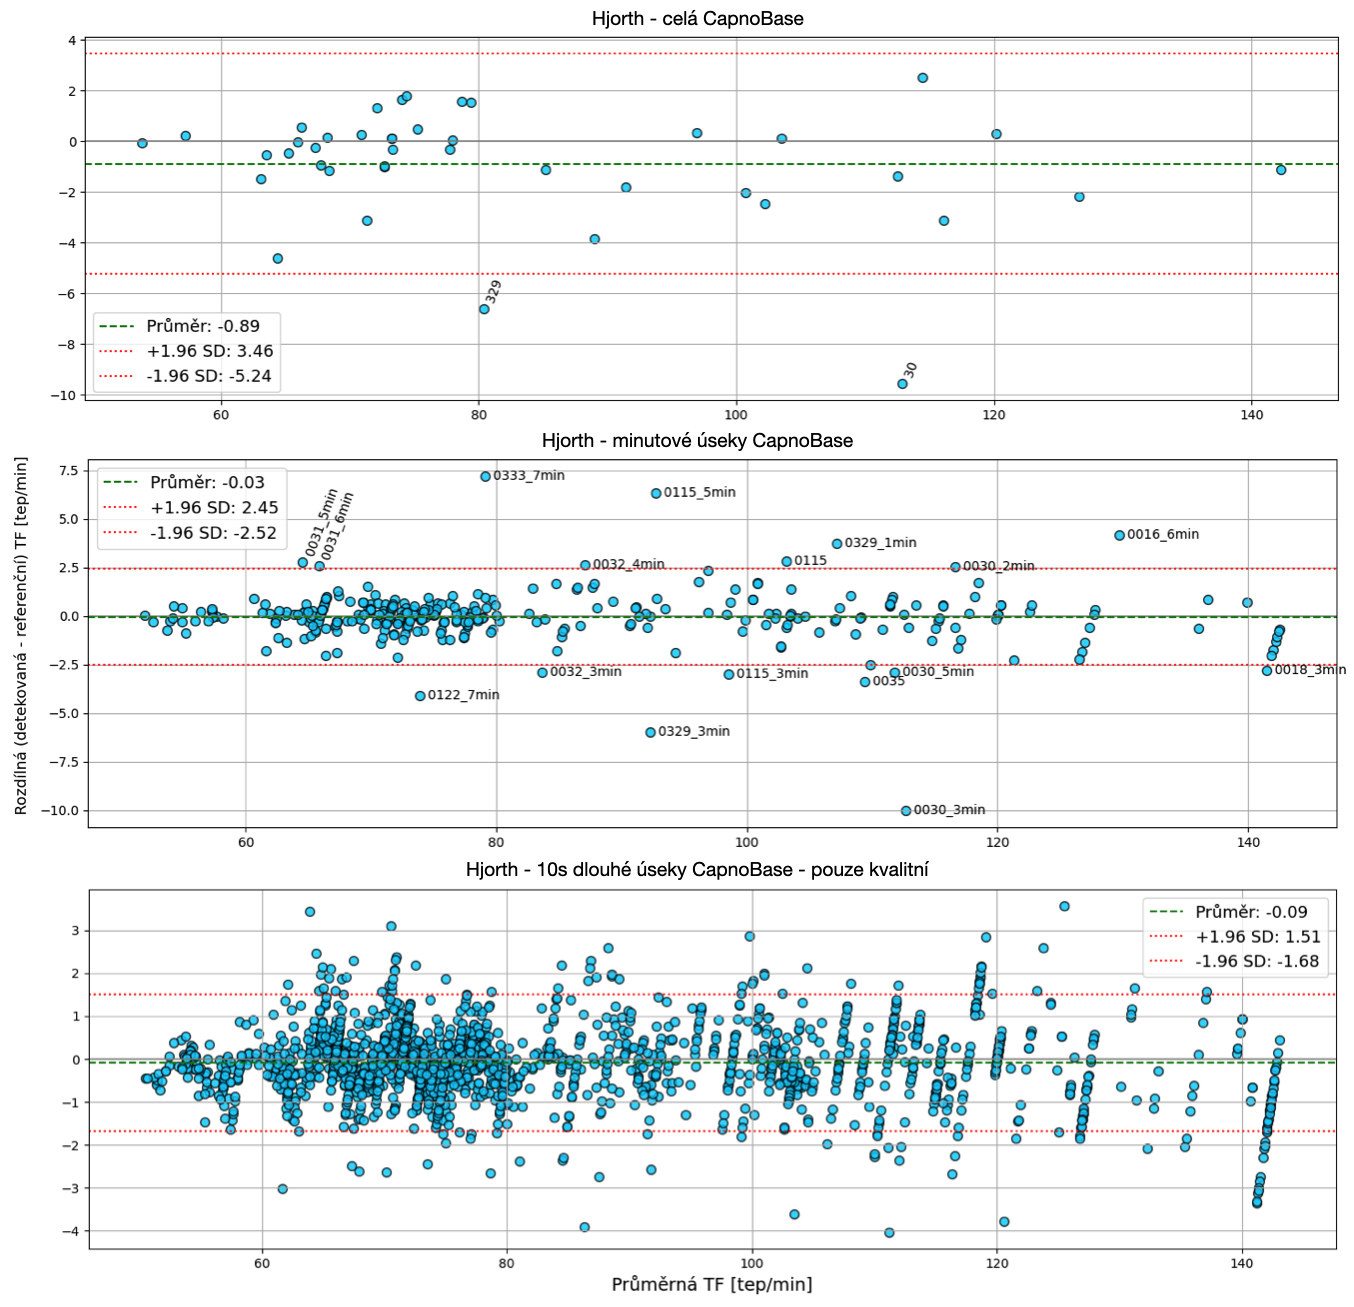
\includegraphics[width=1\textwidth]{./obrazky/vysledky/BlandAltman_CB_Hjorth.png}
	\caption[Bland-Altmanova analýza pro metodu využívající Hjorthovy deskriptory - CapnoBase]{Bland-Altmanova analýza pro metodu využívající Hjorthovy deskriptory.}
	\label{fig:capnobase_BlandAltman_hjorth}
\end{figure}

%%%%%%%%%%%%%%%%%%%%%%%%%%%%%%%%%%%%%%%%%%%%%%%%%%%%%%%%%%%%%%%%%%%
%                             BUT PPG                             %
%%%%%%%%%%%%%%%%%%%%%%%%%%%%%%%%%%%%%%%%%%%%%%%%%%%%%%%%%%%%%%%%%%%
\FloatBarrier
\section{Výsledky pro databázi BUT PPG}
\label{sec:vysledky_butppg}
% Popsat jaké metriky jsme použili pro vyhodnocení kvality detekce TF - už nedetekujeme vrcholy.
Databáze \acs{BUT PPG} neobsahuje referenční anotace systolických vrcholů, a není proto možné vyhodnotit metriky citlivosti (\acs{Se}), přesnosti (\acs{PPV}) ani F1 skóre.
Pro posouzení výkonu jednotlivých algoritmů při odhadu tepové frekvence jsme proto použili průměrnou absolutní chybu (\acs{MAE}) definovanou rovnicí~(\ref{eq:mae}).
Za správně odhadnuté byly považovány ty signály, u nichž byla \acs{MAE} menší než 5~\acs{bpm}, tedy ve shodě s prahovou hodnotou použité již v předchozí podkapitole a doporučenou dle normy IEC~60601-2-27.

Jelikož se v databázi nachází značný počet nekvalitních signálů, byly výsledky interpretovány s ohledem na kvalitu vstupních dat.
K tomu byly využity dvě hodnoty: původní, referenční skóre \acs{R-SQI}, přítomné v metadatech databáze, a dále skóre \acs{O-SQI} získané pomocí algoritmu podle Orphanidou, detailněji popisovaného v~podkapitole~\ref{subsec:referencni_hodnota_kvality}.
Obě hodnoty umožňují binárně rozdělit signály na kvalitní a nekvalitní, což následně slouží k oddělenému hodnocení přesnosti odhadů \acs{TF}.

Souhrnné výsledky pro všechny tři metody odhadu \acs{TF} jsou uvedeny v Tab.~\ref{tab:but_ppg_comparison}.
Výsledky jsou prezentovány ve třech scénářích: pro celou databázi, pro signály označené jako kvalitní na základě \acs{R-SQI} a pro kvalitní signály dle \acs{O-SQI}.
Podobně jako u vyhodnocení databáze CapnoBase jsou kromě hodnoty \acs{MAE} uvedeny také poměry dobře a špatně odhadnutých tepových frekvencí a orientační výpočetní čas algoritmů.

\begin{table}[!ht]
	\centering
	\caption[Srovnání metod odhadu TF na databázi BUT PPG]{Srovnání metod odhadu TF.}
	\label{tab:but_ppg_comparison}
	\resizebox{\textwidth}{!}{
		\begin{tabular}{|l|c|c||c|c||c|c||c|}
			\hline
			\textbf{       } & \multicolumn{2}{|c|}{\textbf{celá databáze}} & \multicolumn{2}{|c|}{\textbf{\acs{R-SQI}}}  & \multicolumn{2}{|c|}{\textbf{\acs{O-SQI}}} &  \\
			\hline
			\textbf{       } &     \textbf{MAE}     & \textbf{Poměr} &     \textbf{MAE}     & \textbf{Poměr} &     \textbf{MAE}     & \textbf{Poměr} & \textbf{Čas} \\
			\textbf{Metoda}  & \textbf{[\acs{bpm}]} & \textbf{[d:š]} & \textbf{[\acs{bpm}]} & \textbf{[d:š]} & \textbf{[\acs{bpm}]} & \textbf{[d:š]} & \textbf{[s]} \\
			\hline\hline
			Elgendi          &  18,84  & 875\textbf{:}2.797 &  6,73   &  511\textbf{:}299  &  7,82  &  177\textbf{:}90  &  x  \\
			\hline
			Vlastní          &         &                    &         &                    &        &                   &     \\
			vrcholová        &  20,54  & 875\textbf{:}2.797 &  7,80   &  507\textbf{:}303  &  7,12  &  183\textbf{:}84  &  x  \\
			detekce          &         &                    &         &                    &        &                   &     \\
			\hline
			Hjorth           &  31,22  & 624\textbf{:}3.048 &  12,98  &  497\textbf{:}313  &  8,05  &  182\textbf{:}85  &  x  \\
			\hline
		\end{tabular}
		}
\end{table}

\begin{figure}[!ht]
	\centering
	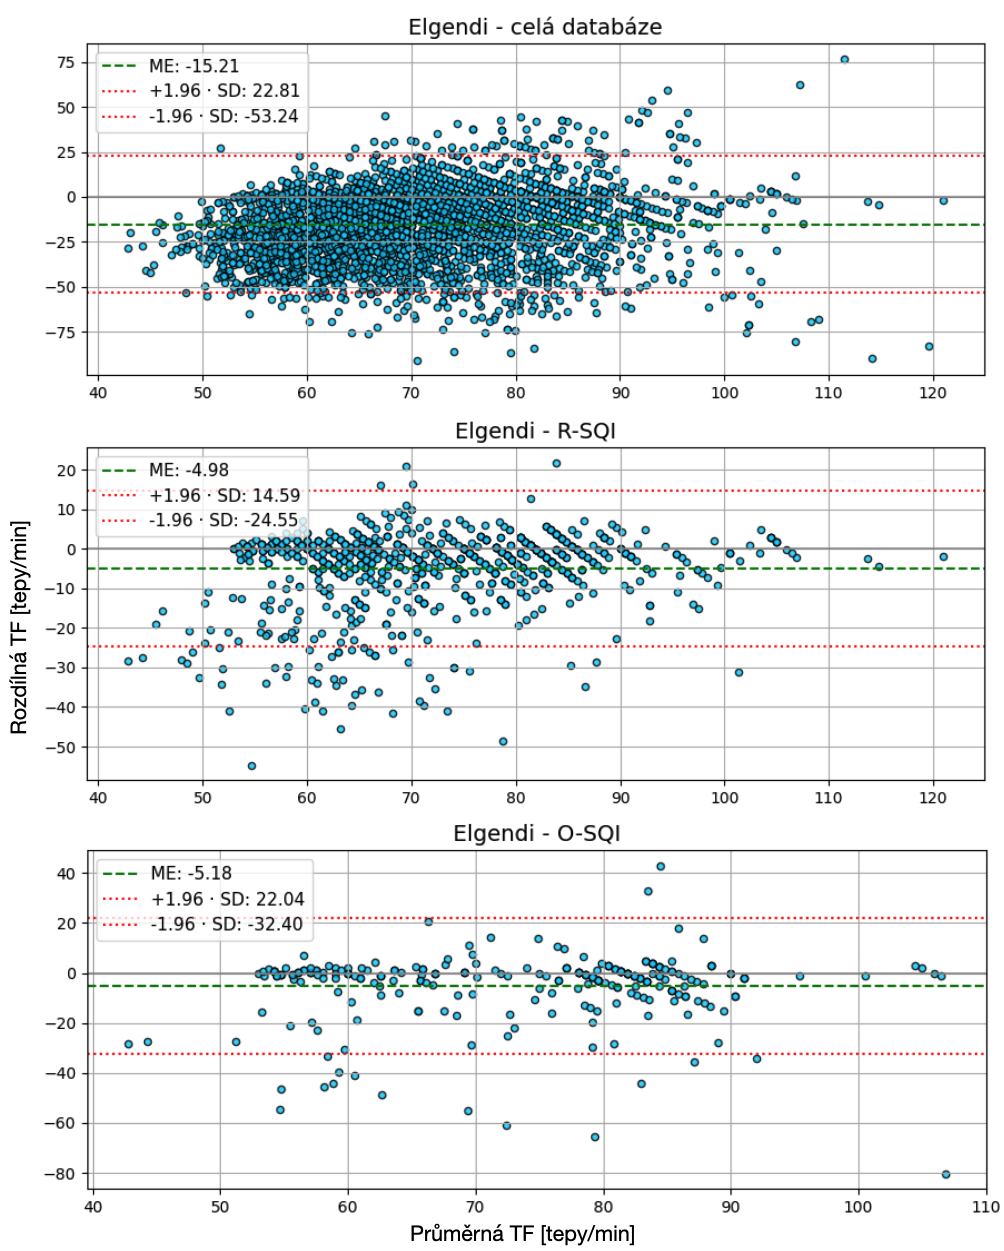
\includegraphics[width=1\textwidth]{./obrazky/vysledky/BA_BUT_Elgendi.png}
	\caption[Bland-Altmanova analýza pro Elgendiho metodu - BUT PPG]{Bland-Altmanova analýza pro Elgendiho metodu.}
	\label{fig:BUT_BlandAltman_elgendi}
\end{figure}

\begin{figure}[!ht]
	\centering
	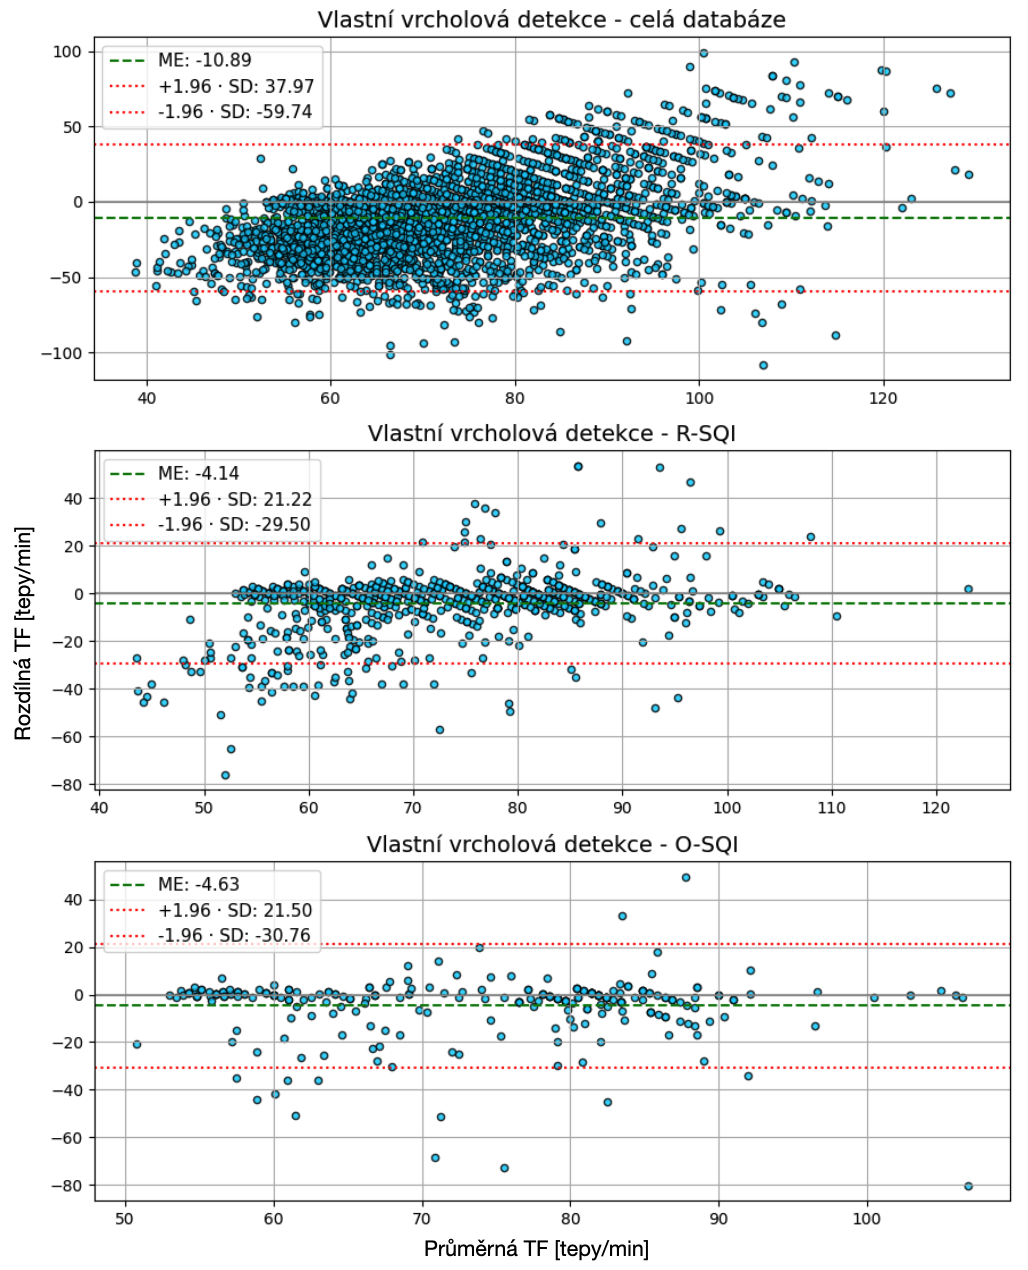
\includegraphics[width=1\textwidth]{./obrazky/vysledky/BA_BUT_VVD.png}
	\caption[Bland-Altmanova analýza pro naši metodu detekující vrcholy - BUT PPG]{Bland-Altmanova analýza pro naši metodu detekující vrcholy.}
	\label{fig:BUT_BlandAltman_vvd}
\end{figure}

\begin{figure}[!ht]
	\centering
	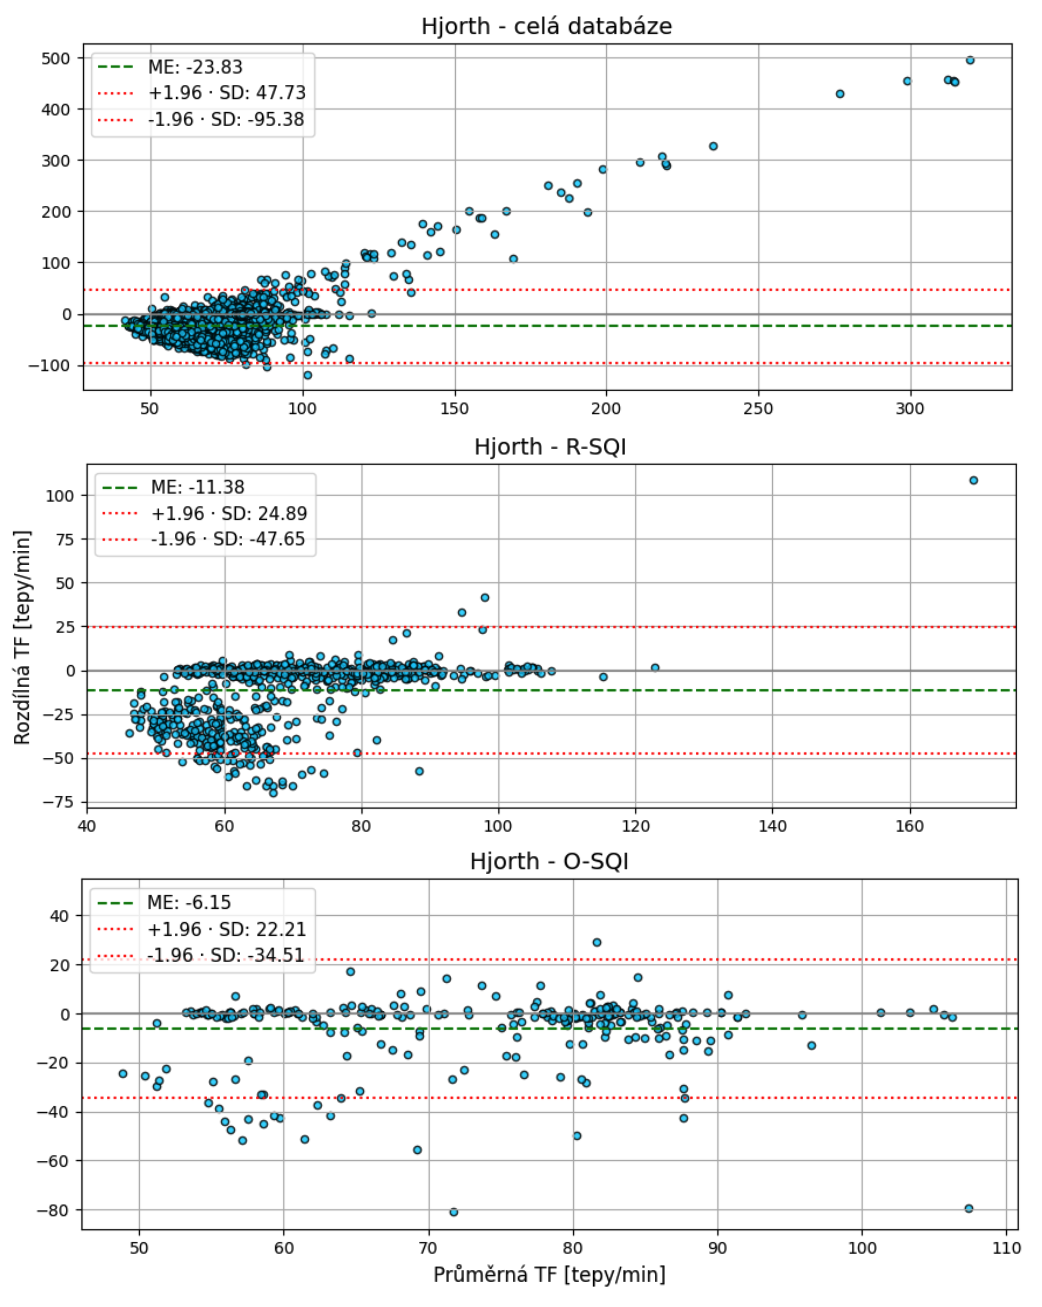
\includegraphics[width=1\textwidth]{./obrazky/vysledky/BA_BUT_Hjorth.png}
	\caption[Bland-Altmanova analýza pro metodu využívající Hjorthovy deskriptory - BUT PPG]{Bland-Altmanova analýza pro metodu využívající Hjorthovy deskriptory.}
	\label{fig:BUT_BlandAltman_hjorth}
\end{figure}

%%%%%%%%%%%%%%%%%%%%%%%%%%%%%%%%%%%%%%%%%%%%%%%%%%%%%%%%%%%%%%%%%%%
%                             Kvalita                             %
%%%%%%%%%%%%%%%%%%%%%%%%%%%%%%%%%%%%%%%%%%%%%%%%%%%%%%%%%%%%%%%%%%%
\FloatBarrier
\section{Výsledky automatického posouzení kvality}
\label{sec:vysledky_kvalita}

%%% Vložení souboru 'text/diskuze' s diskuzí výsledků
\chapter{Diskuze} % Vysvětluje, co výsledky znamenají
\label{ch:diskuze}
% Interpretace výsledků = co znamenají.
% Porovnání s literaturou: odpovídají výsledky očekáváním? V čem se liší?
% Vysvětlení možných příčin, omezení, nejistot, překvapení.
% Reflexe metod: byly vhodně zvoleny? Co by šlo udělat lépe?
% Možné dopady, návrhy pro budoucí výzkum.

% - „Tento výsledek může být způsoben tím, že…“,
% - „Na rozdíl od práce XY jsme zaznamenali…“,
% - „Překvapivě model selhal při…“
Z~grafů je patrné, že až na několik málo odchylek u~jednotlivých signálů dosahují obě metody v~průměru vysokých hodnot \acs{Se} i \acs{PPV}.

Na Obr.~\ref{fig:capnobase_our_err} došlo k~selhání detekce z~důvodu přítomnosti silné respirační vlny.

% V BA analýze se na osu $x$ obvykle klade průměr hodnot získaných oběma metodami (zde: referenční a odhadnutá TF).
% Důvodem je, že chyby mohou být závislé na velikosti měřené veličiny – tedy chceme vidět, zda se chyba mění se vzrůstající hodnotou.
% = to je pravda, diskutujme to.

% Bland-Altmanova analýza nám umožňuje posoudit, jak výrazně se odhady liší od referenčních hodnot a zda je chyba závislá na velikosti tepové frekvence.


%%% Vložení souboru 'text/zaver' se závěrem
\chapter*{Závěr}
\phantomsection
\addcontentsline{toc}{chapter}{Závěr}

% !? Jak později v práci správně psát zkratky?
Tato bakalářská práce se zaměřila na odhad tepové frekvence (\acs{TF}) z fotopletysmografických (\acs{PPG}) signálů.
Cílem bylo jednak poskytnout stručný přehled existujících metod pro odhad TF z PPG signálů, jednak navrhnout a popsat algoritmy pro spolehlivé stanovení tepové frekvence.

V teoretické části byla popsána fotopletysmografie jako neinvazivní optická metoda monitorování změn objemu krve v tkáních, která se používá zejména pro sledování kardiovaskulárních parametrů.
Byly představeny základní principy PPG signálů a faktory, které mohou ovlivnit jejich kvalitu a přesnost měření.

Praktická část práce se soustředila na implementaci a testování několika algoritmů pro detekci systolických vrcholů v PPG signálech, včetně Aboyova algoritmu, jeho vylepšené verze Aboy++, Elgendiho algoritmu, Rezonátoru s nulovou frekvencí (ZFR) a nově navrženého Upraveného Aboyova algoritmu.
Algoritmy byly testovány na dvou databázích: CapnoBase a BUT PPG.

Výsledky ukázaly, že Rezonátor s nulovou frekvencí (ZFR) dosahuje nejlepších výsledků na databázi CapnoBase, přičemž vykazuje vysokou citlivost a pozitivní prediktivní hodnotu.
Elgendiho algoritmus se prokázal jako nejspolehlivější na databázi BUT PPG, přičemž dosahoval nejnižší průměrné odchylky mezi detekovanou a referenční TF.

Jedním z klíčových cílů této práce byl vývoj a implementace upraveného Aboyova algoritmu.
Tento algoritmus dosahuje lepších odhadů TF na databázi CapnoBase ve srovnání s původní verzí, a to zejména díky zjednodušení a odstranění některých kroků, které způsobovaly přehlížení skutečných systolických vrcholů.
Na databázi BUT PPG však vykazoval vyšší odchylky TF, což naznačuje potřebu další optimalizace pro spolehlivější detekci.

Dalším krokem pro zlepšení přesnosti odhadu TF by mohlo být využití pokročilejších technik strojového učení a hlubokých neuronových sítí, které mohou nabídnout lepší adaptaci na různé typy signálů a zlepšit robustnost algoritmů vůči šumu a artefaktům.


%%% Vložení souboru 'text/literatura' se seznamem zdrojů
% Pro sazbu seznamu literatury použijte jednu z následujících možností

%%%%%%%%%%%%%%%%%%%%%%%%%%%%%%%%%%%%%%%%%%%%%%%%%%%%%%%%%%%%%%%%%%%%%%%%%
%1) Seznam citací definovaný přímo pomocí prostředí literatura / thebibliography

\begin{thebibliography}{99}

	%%%%%%%%%%%%%%%%%%%%%%%%%%%%%%%%%%%%%%%%%%%%%%%%%%%%%%%%%%%%%%%%%%%%%
	%%%%%%%%%%%%%%%%%%%%%%%%%%%%% Databases %%%%%%%%%%%%%%%%%%%%%%%%%%%%%
	%%%%%%%%%%%%%%%%%%%%%%%%%%%%%%%%%%%%%%%%%%%%%%%%%%%%%%%%%%%%%%%%%%%%%
	\bibitem{BUT_PPG}
		NEMCOVA, Andrea, Enikö VARGOVA, Radovan SMISEK, Lucie MARSANOVA, Lukas SMITAL, Martin VITEK a Mihajlo JAKOVLJEVIC.
		Brno University of Technology Smartphone PPG Database (BUT PPG): Annotated Dataset for PPG Quality Assessment and Heart Rate Estimation.
		\emph{BioMed Research International} [online].
		2021-09-06, 2021, 1-6 [cit. 2024-05-23].
		ISSN 2314-6141.
		Dostupné z: \url{https://doi.org/10.1155/2021/3453007}

	\bibitem{BUT_PPG_database}
		Nemcova, A., Smisek, R., Vargova, E., Maršánová, L., Vitek, M., Smital, L., Filipenska, M., Sikorova, P., a Gálík, P.
		Brno University of Technology Smartphone PPG Database (BUT PPG) (version 2.0.0).
		PhysioNet.
		2024 [cit. 2025-03-23].
		Dostupné z: \url{https://doi.org/10.13026/tn53-8153}

	\bibitem{CapnoBase}
		KARLEN, Walter.
		CapnoBase IEEE TBME Respiratory Rate Benchmark.
		\emph{Borealis} [online].
		2021 [cit. 2024-05-23].
		Dostupné z: \url{https://doi.org/10.5683/SP2/NLB8IT}

	% \bibitem{Karlen2013-CB}
	% 	KARLEN, Walter, S. RAMAN, J. M. ANSERMINO a G. A. DUMONT.
	% 	Multiparameter respiratory rate estimation from the photoplethysmogram.
	% 	\emph{IEEE Transactions on Biomedical Engineering}.
	% 	2013, 60(7), 1946-1953.
	% 	DOI: \url{https://doi.org/10.1109/TBME.2013.2246160}

	%%%%%%%%%%%%%%%%%%%%%%%%%%%%%%%%%%%%%%%%%%%%%%%%%%%%%%%%%%%%%%%%%%%%%
	%%%%%%%%%%%%% TECHNICKÁ - PRAKTICKÁ - PROGRAMOVACÍ ČÁST %%%%%%%%%%%%%
	%%%%%%%%%%%%%%%%%%%%%%%%%%%%%%%%%%%%%%%%%%%%%%%%%%%%%%%%%%%%%%%%%%%%%
	\bibitem{ENIKÖ}
		VARGOVÁ, Enikö.
		\emph{Stanovení kvality a odhad tepové frekvence ze signálu PPG} [online].
		Brno, 2021 [cit. 2022-11-15].
		Dostupné z: \url{https://www.vutbr.cz/studenti/zav-prace/detail/134388}.
		Bakalářská práce. Vysoké učení technické v Brně, Fakulta elektrotechniky a komunikačních technologií, Ústav biomedicínského inženýrství.
		Vedoucí práce Andrea Němcová.

	\bibitem{Siddiqui2016}	% dostupné jen na webu
		SIDDIQUI, Sarah Ali, Yuan ZHANG, Zhiquan FENG a Anton KOS.
		A Pulse Rate Estimation Algorithm Using PPG and Smartphone Camera.
		\emph{Journal of Medical Systems} [online].
		2016, 40(5) [cit. 2024-05-20].
		ISSN 0148-5598.
		Dostupné z: \url{https://doi.org/10.1007/s10916-016-0485-6}

	\bibitem{Charlton2022}
		CHARLTON, Peter H, Kevin KOTZEN, Elisa MEJÍA-MEJÍA, et al.
		Detecting beats in the photoplethysmogram: benchmarking open-source algorithms.
		\emph{Physiological Measurement} [online].
		2022-08-19, 43(8) [cit. 2024-05-20].
		ISSN 0967-3334.
		Dostupné z: \url{https://doi.org/10.1088/1361-6579/ac826d}

	% Popis nositelných zařízení a jejich využití měřící PPG
	% - SENZOR DESIGN - SIGNAL PROCESSING - APPLICATIONS - RESEARCH DIRECTIONS
	\bibitem{Charlton2023}
		CHARLTON, Peter H, John ALLEN, Raquel BAILÓN, et al.
		The 2023 wearable photoplethysmography roadmap.
		\emph{Physiological Measurement} [online].
		2023-11-29, 44(11) [cit. 2024-05-20].
		ISSN 0967-3334.
		Dostupné z: \url{https://doi.org/10.1088/1361-6579/acead2}

	\bibitem{Karlen2013}	% šlo by se zbavit této citace?
		KARLEN, Walter, S. RAMAN, J. M. ANSERMINO a G. A. DUMONT.
		Multiparameter Respiratory Rate Estimation From the Photoplethysmogram.
		\emph{IEEE Transactions on Biomedical Engineering} [online].
		2013, 60(7), 1946-1953 [cit. 2024-04-16].
		ISSN 0018-9294.
		Dostupné z: \url{https://doi.org/10.1109/TBME.2013.2246160}

	% Kvalita signálu - popis PPG - detekce TF
	\bibitem{Orphanidou2015}
		ORPHANIDOU, Christina, Timothy BONNICI, Peter CHARLTON, David CLIFTON, David VALLANCE a Lionel TARASSENKO.
		Signal-Quality Indices for the Electrocardiogram and Photoplethysmogram: Derivation and Applications to Wireless Monitoring.
		\emph{IEEE Journal of Biomedical and Health Informatics} [online].
		2015, (3), 832-838 [cit. 2025-04-20].
		Dostupné z: \url{https://doi.org/10.1109/JBHI.2014.2338351}

	\bibitem{Orphanidou2018}
		ORPHANIDOU, Christina.
		\emph{Signal Quality Assessment in Physiological Monitoring} [online].
		Cham: Springer International Publishing, 2018 [cit. 2024-05-20].
		SpringerBriefs in Bioengineering.
		ISBN 978-3-319-68414-7.
		Dostupné z: \url{https://doi.org/10.1007/978-3-319-68415-4}

	\bibitem{PyPPG}
		GODA, Márton Á, Peter H CHARLTON a Joachim A BEHAR.
		pyPPG: A Python toolbox for comprehensive photoplethysmography signal analysis.
		\emph{Physiological Measurement} [online].
		2024-04-08, 45(4) [cit. 2024-05-20].
		ISSN 0967-3334.
		Dostupné z: \url{https://doi.org/10.1088/1361-6579/ad33a2}

	\bibitem{Pribil2023AnalysisOH}
		PŘIBIL, Jiří, Anna PŘIBILOVÁ a Ivan FROLLO.
		Analysis of Heart Pulse Transmission Parameters Determined from Multi-Channel PPG Signals Acquired by a Wearable Optical Sensor.
		\emph{Measurement Science Review} [online].
		2023, 23, 217-226 [cit. 2025-2-20].
		Dostupné z: \url{https://api.semanticscholar.org/CorpusID:264289667}

	% NeuroKit2
	\bibitem{Elgendi2013}
		ELGENDI, Mohamed, Ian NORTON, Matt BREARLEY, Derek ABBOTT, Dale SCHUURMANS a Vladimir E. BONDARENKO.
		Systolic Peak Detection in Acceleration Photoplethysmograms Measured from Emergency Responders in Tropical Conditions.
		\emph{PLoS ONE} [online].
		2013-10-22, 8(10) [cit. 2024-05-20].
		ISSN 1932-6203.
		Dostupné z: \url{https://doi.org/10.1371/journal.pone.0076585}

	\bibitem{NeuroKit2}
		MAKOWSKI, Dominique, Tam Pham, Zuo Jia Lau, et al.
		NeuroKit2: A Python toolbox for neurophysiological signal processing.
		\emph{Behavior Research Methods} [online].
		2021, 53, 1689–1696 [cit. 2024-05-20].
		ISSN 1554-3528.
		Dostupné z: \url{https://doi.org/10.3758/s13428-020-01516-y}

	% Hjorth
	\bibitem{Hjorth1970}
		HJORTH, Bo.
		EEG analysis based on time domain properties.
		\emph{Electroencephalography and Clinical Neurophysiology} [online].
		1970, 29, 306-310 [cit. 2025-04-23].
		Dostupné z: \url{https://doi.org/10.1016/0013-4694(70)90143-4}

	\bibitem{Hjorth1973}
		HJORTH, Bo.
		The physical significance of time domain descriptors in EEG analysis.
		\emph{Electroencephalography and Clinical Neurophysiology} [online].
		1973, 34(3), 321-325 [cit. 2025-04-14].
		ISSN 00134694.
		Dostupné z: \url{https://doi.org/10.1016/0013-4694(73)90260-5}

	\bibitem{Peralta2017}
		PERALTA, Elena, Jesus LAZARO, Eduardo GIL, Raquel BAILÓN a Vaidotas MAROZAS.
		Robust Pulse Rate Variability Analysis from Reflection and Transmission Photoplethysmographic Signals [online].
		2017-09-14, - [cit. 2025-04-10].
		Dostupné z: \url{https://doi.org/10.22489/CinC.2017.205-286}

	\bibitem{Geetika2022}
		KAUSHIK, Geetika, Pramod GAUR, Rishi Raj SHARMA a Ram Bilas PACHORI.
		EEG signal based seizure detection focused on Hjorth parameters from tunable-Q wavelet sub-bands.
		\emph{Biomedical Signal Processing and Control} [online].
		2022, 76 [cit. 2024-04-20].
		ISSN 1746-8094.
		Dostupné z: \url{https://doi.org/10.1016/j.bspc.2022.103645}

	%%%%%%%%%%%%%%%%%%%%%%%%%%%%%%%%%%%%%%%%%%%%%%%%%%%%%%%%%%%%%%%%%%%%%
	%%%%%%%%%%%%%%%%%%%%%%%%% FYZIOLOGICKÁ ČÁST %%%%%%%%%%%%%%%%%%%%%%%%%
	%%%%%%%%%%%%%%%%%%%%%%%%%%%%%%%%%%%%%%%%%%%%%%%%%%%%%%%%%%%%%%%%%%%%%
	\bibitem{ucebniceFyziologie}	% dostupné jen v knihovně
		MOUREK, Jindřich.
		\emph{Fyziologie: učebnice pro studenty zdravotnických oborů.}
		2.\, dopl. vydání Praha: Grada. Sestra (Grada), 2012.
		ISBN 978-80-247-3918-2

	\bibitem{vnitrniLekarstviVKostce}	% dostupné jen v papírové podobě
		SOUČEK, Miroslav, Petr SVAČINA a kolektiv.
		\emph{Vnitřní lékařství v kostce.}
		Praha: Grada Publishing, 2019.
		ISBN 978-80-271-2289-9.

	\bibitem{faktoryOvlivnujiciTep}	% šlob by se zbavit této citace?
		GONZAGA, Luana Almeida, Luiz Carlos Marques VANDERLEI, Rayana Loch GOMES a Vitor Engrácia VALENTI.
		Caffeine affects autonomic control of heart rate and blood pressure recovery after aerobic exercise in young adults: a crossover study.
		\emph{Scientific Reports} [online].
		2017, 7(1) [cit. 2024-05-15].
		ISSN 2045-2322.
		Dostupné z: \url{https://doi.org/10.1038/s41598-017-14540-4}

	% Přehledový článek o analýze PPG a jejích aplikacích
	\bibitem{Park2022}
		PARK, Junyung, Hyeon Seok SEOK, Sang-Su KIM a Hangsik SHIN.
		Photoplethysmogram Analysis and Applications: An Integrative Review.
		\emph{Frontiers in Physiology} [online].
		2022-03-01, 12 [cit. 2022-12-18].
		ISSN 1664-042X.
		Dostupné z: \url{https://doi.org/10.3389/fphys.2021.808451}

	% Přehledový článek o využití PPG v praxi
	\bibitem{PoveaCabrera2018}
		POVEA, Camilo E. a Arturo CABRERA.
		Practical usefulness of heart rate monitoring in physical exercise.
		\emph{Revista Colombiana de Cardiología} [online].
		2018, 25(3), e9-e13 [cit. 2024-05-15].
		ISSN 01205633.
		Dostupné z: \url{https://doi.org/10.1016/j.rccar.2018.05.004}


	%%%%%%%%%%%%%%%%%%%%%%%%%%%%%%%%%%%%%%%%%%%%%%%%%%%%%%%%%%%%%%%%%%%%%
	%%%%%%%%%%%%%%%%%%%%%%%%%% NORMY A PŘEDPISY %%%%%%%%%%%%%%%%%%%%%%%%%
	%%%%%%%%%%%%%%%%%%%%%%%%%%%%%%%%%%%%%%%%%%%%%%%%%%%%%%%%%%%%%%%%%%%%%
	\bibitem{CSN_ISO_690-2022}
		ÚŘAD PRO TECHNICKOU NORMALIZACI, METROLOGII A~STÁTNÍ ZKUŠEBNICTVÍ.
		ČSN ISO 690:2022 (01 0197), \emph{Informace a dokumentace -- Pravidla pro bibliografické odkazy a~citace informačních zdrojů.}
		Čtvrté vydání. Praha, 2022.

	\bibitem{CSN_ISO_7144-1997}
		ÚŘAD PRO TECHNICKOU NORMALIZACI, METROLOGII A~STÁTNÍ ZKUŠEBNICTVÍ.
		ČSN ISO 7144 (010161), \emph{Dokumentace -- Formální úprava disertací a~podobných dokumentů.}
	%	24 stran.
		Praha, 1997.

	\bibitem{CSN_ISO_31-11}
		ÚŘAD PRO TECHNICKOU NORMALIZACI, METROLOGII A~STÁTNÍ ZKUŠEBNICTVÍ.
		ČSN ISO 31-11, \emph{Veličiny a~jednotky -- část 11: Matematické znaky a~značky používané ve fyzikálních vědách a~v~technice.}
		Praha, 1999.

	\bibitem{Farkasova23:CSNISO6902022komentar}
		FARKAŠOVÁ, B.; GARAMSZEGI T.; JANSOVÁ L.; KONEČNÝ L.; KRČÁL M.\ et~al.
		\emph{Výklad normy ČSN ISO 690:2022 (01 0197) účinné od 1.\,12.\,2022}.
		Online. První vydání. 2023.
		Dostupné~z:
		\url{https://www.citace.com/Vyklad-CSN-ISO-690-2022.pdf}.
		[cit.\,2023-09-27].

\end{thebibliography}


%%%%%%%%%%%%%%%%%%%%%%%%%%%%%%%%%%%%%%%%%%%%%%%%%%%%%%%%%%%%%%%%%%%%%%%%%
%%2) Seznam citací pomocí BibTeXu
%% Při použití je nutné v TeXnicCenter ve výstupním profilu aktivovat spouštění BibTeXu po překladu.
%% Definice stylu seznamu
%\bibliographystyle{unsrturl}
%% Pro českou sazbu lze použít styl czechiso.bst ze stránek
%% http://www.fit.vutbr.cz/~martinek/latex/czechiso.tar.gz
%%\bibliographystyle{czechiso}
%% Vložení souboru se seznamem citací
%\bibliography{text/literatura}
%
%% Následující příkaz je pouze pro ukázku sazby literatury při použití BibTeXu.
%% Způsobí citaci všech zdrojů v souboru literatura.bib, i když nejsou citovány v textu.
%\nocite{*}

%%% Vložení souboru 'text/10_zkratky' se seznam použitých symbolů, veličin a zkratek
\cleardoublepage
\chapter*{\listofabbrevname}
\phantomsection
\addcontentsline{toc}{chapter}{\listofabbrevname}

\begin{acronym}[KolikMista]	% [KolikMista] určuje šířku sloupce pro zkratky, je to maximální délka zkratky

	\acro{symfvz}
		[\ensuremath{f_\textind{vz}}]
		{vzorkovací kmitočet}

	\acro{VUT}		{Vysoké učení technické v Brně}
	\acro{CESA}		{Centrum sportovních aktivit}
	\acro{FEKT}		{Fakulta elektrotechniky a komunikačních technologií}

	\acro{BUT PPG}	{Brno University of Technology Smartphone PPG Database}
	\acro{WFDB}		{WaveForm Database}

	\acro{PPG}		{Fotopletysmograf}
	\acro{EKG}		{Elektrokardiogram}
	\acro{EEG}		{Elektroencefalogram}
	\acro{ACC}		{Akcelerometr}

	\acro{TF}		{Tepová frekvence}
	\acro{MTF}		{Maximální tepová frekvence}
	\acro{IBI}		{Tepový interval}

	\acro{LED}		{Elektroluminiscenční dioda}

	\acro{DC}		{Stejnostměrná složka}

	\acro{MA}		{klouzavý průměr}
	\acro{MA_P}
		[\ensuremath{\var{MA}_\textind{peak}}]
			{klouzavý průměr pro zvýraznění vrcholu}
	\acro{MA_B}
		[\ensuremath{\var{MA}_\textind{beat}}]
		{klouzavý průměr pro zvýraznění tepu}
	\acro{THR_1}
		[\ensuremath{\var{THR}_\textind{1}}]
		{práh 1}
	\acro{THR_2}
		[\ensuremath{\var{THR}_\textind{2}}]
		{práh 2}
	
	% \acro{FIR}		{Filtr s konečnou impulzní charakteristikou}
	% \acro{IIR}		{Filtr s nekonečnou impulzní charakteristikou}
	\acro{FFT}		{Rychlá Fourierova transformace}

	\acro{RF}		{Náhodný les}

	\acro{H_0}
		[\ensuremath{\var{H}_\textind{0}}]
		{Aktivita}
	\acro{H_1}
		[\ensuremath{\var{H}_\textind{1}}]
		{Mobilita}
	\acro{H_2}
		[\ensuremath{\var{H}_\textind{2}}]
		{Komplexita}
	\acro{SPI}		{Index spektrální čistoty}

	\acro{TN}		{Pravdivě negativní}
	\acro{TP}		{Pravdivě pozitivní}
	\acro{FN}		{Falešně negativní}
	\acro{FP}		{Falešně pozitivní}

	\acro{PPV}		{Pozitivní prediktivní hodnota}
	\acro{Se}		{Citlivost}
	\acro{F1}		{F1 skóre}
	\acro{MAE}		{Průměrná absolutní chyba}
	\acro{RMSE}		{Průměrná kvadratická chyba}

	\acro{var}		{rozptyl}

	\acro{Hz}		{Hertz}
	% \acro{rad}		{Radián}
	\acro{ms}		{Milisekunda}
	\acro{s}		{Sekunda}
	% \acro{min}		{Minuta}

	% \acro{ZFR}		{Rezonátor s nulovou frekvencí}

\end{acronym}


%%% Začátek příloh
% \appendix

%%% Vysázení seznamu příloh
% (vynechejte, pokud máte dvě nebo méně příloh)
% \listofappendices

%%% Vložení souboru 'text/prilohy' s přílohami
% Obvykle je přítomen alespoň popis co najdeme na přiloženém médiu
% \chapter{Některé příkazy balíčku \texttt{thesis}}

\section{Příkazy pro sazbu veličin a jednotek}

\begin{table}[!h]
  \caption[Přehled příkazů]{Přehled příkazů pro matematické prostředí }
  \begin{center}
  	\small
	  \begin{tabular}{|c|c|c|c|}
	    \hline
	    Příkaz    						& Příklad 					& Zdroj příkladu  							& Význam  \\
	    \hline\hline
	    \verb|\textind{...}|	& $\beta_\textind{max}$ 	& \verb|$\beta_\textind{max}$|	& textový index \\
	    \hline
	    \verb|\const{...}| 		& $\const{U}_\textind{in}$ 				& \verb|$\const{U}_\textind{in}$|		& konstantní veličina \\
	    \hline
	    \verb|\var{...}| 		& $\var{u}_\textind{in}$ & \verb|$\var{u}_\textind{in}$| & proměnná veličina \\
	    \hline
	    \verb|\complex{...}| 	& $\complex{u}_\textind{in}$ & \verb|$\complex{u}_\textind{in}$| & komplexní veličina \\
	    \hline
	    \verb|\vect{...}| 		& $\vect{y}$ 						& \verb|$\vect{y}$| & vektor \\
	    \hline
	    \verb|\mat{...}| 	& $\mat{Z}$ 						& \verb|$\mat{Z}$| & matice \\
	    \hline
	    \verb|\unit{...}| 		& $\unit{kV}$ 						& \verb|$\unit{kV}$|\quad či\ \, \verb|\unit{kV}| & jednotka \\
	    \hline
	  \end{tabular}
  \end{center}
\end{table}



%\newpage
\section{Příkazy pro sazbu symbolů}

\begin{itemize}
  \item
    \verb|\E|, \verb|\eul| -- sazba Eulerova čísla: $\eul$,
  \item
    \verb|\J|, \verb|\jmag|, \verb|\I|, \verb|\imag| -- sazba imaginární jednotky: $\jmag$, $\imag$,
  \item
    \verb|\dif| -- sazba diferenciálu: $\dif$,
  \item
    \verb|\sinc| -- sazba funkce: $\sinc$,
  \item
    \verb|\mikro| -- sazba symbolu mikro stojatým písmem%
			\footnote{znak pochází z~balíčku \texttt{textcomp}}: $\mikro$,
	\item
		\verb|\uppi| -- sazba symbolu $\uppi$
			(stojaté řecké pí, na rozdíl od \verb|\pi|, což sází $\pi$).
\end{itemize}
%
Všechny symboly jsou určeny pro matematický mód, vyjma \verb|\mikro|, jenž je\\ použitelný rovněž v~textovém módu.
%$\upmikro$


\chapter{Druhá příloha}

\begin{figure}[!h]
  \begin{center}
    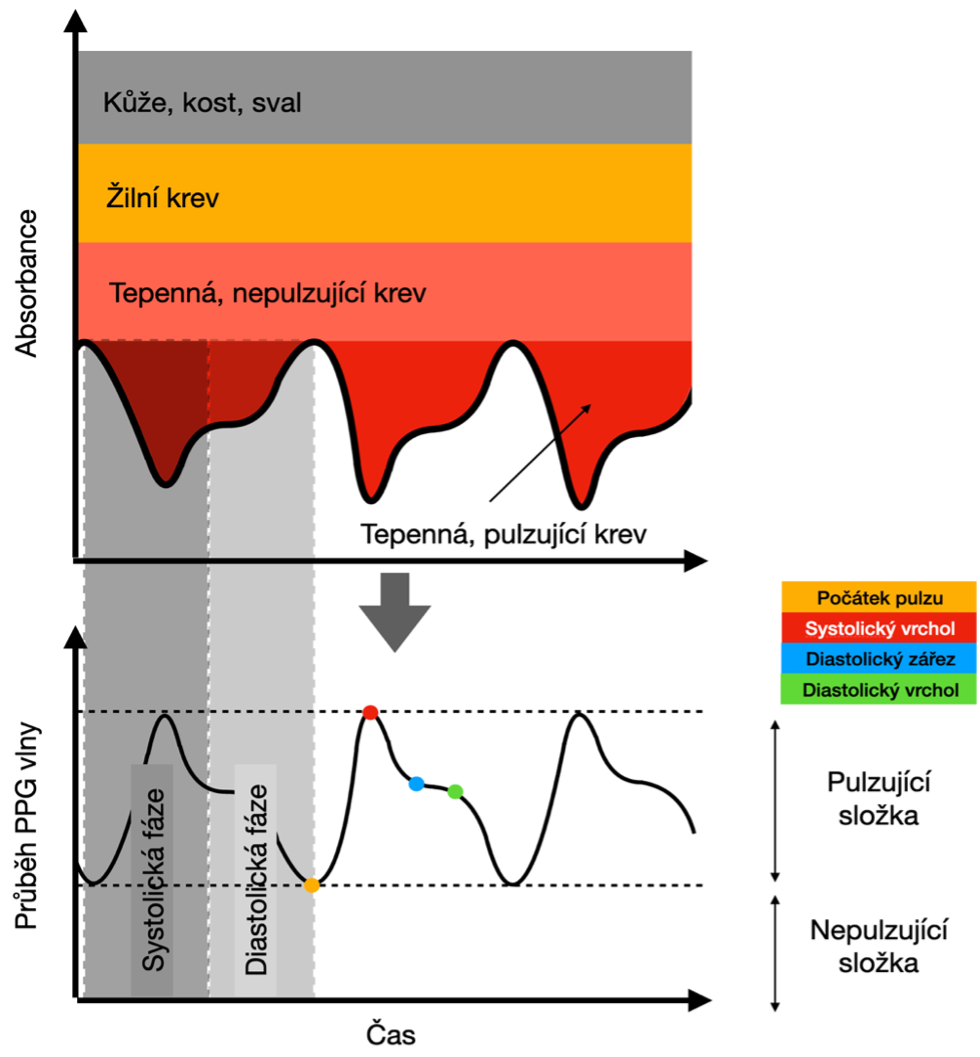
\includegraphics[scale=0.5]{obrazky/signalPPG.png}
  \end{center}
  \caption[Origo Template]{Signál PPG.}
\end{figure}

Pro sazbu vektorových obrázků přímo v~\LaTeX{}u je možné doporučit balíček \href{https://www.ctan.org/pkg/pgf}{\texttt{TikZ}}.
Příklady sazby je možné najít na \href{http://www.texample.net/tikz/examples/}{\TeX{}ample}.
Pro vyzkoušení je možné použít programy QTikz nebo TikzEdt.




\chapter{Příklad sazby zdrojových kódů}

\section{Balíček \texttt{listings}}

Pro vysázení zdrojových souborů je možné použít balíček \href{https://www.ctan.org/pkg/listings}{\texttt{listings}}.
Balíček zavádí nové prostředí \texttt{lstlisting} pro sazbu zdrojových kódů, jako například:
%
\begin{lstlisting}[language={[LaTeX]TeX}]
\section{Balíček lstlistings}
Pro vysázení zdrojových souborů je možné použít
	balíček \href{https://www.ctan.org/pkg/listings}%
	{\texttt{listings}}.
Balíček zavádí nové prostředí \texttt{lstlisting} pro
	sazbu zdrojových kódů.
\end{lstlisting}
%
Podporuje množství programovacích jazyků.
Kód k~vysázení může být načítán přímo ze zdrojových souborů.
Umožňuje vkládat čísla řádků nebo vypisovat jen vybrané úseky kódu.
Např.:

\noindent
Zkratky jsou sázeny v~prostředí \texttt{acronym}:
\label{lst:zkratky}
\lstinputlisting[language={[LaTeX]TeX},nolol,numbers=left, firstnumber=6, firstline=6,lastline=6]{text/98_zkratky.tex}
%
Šířka textu volitelného parametru \verb|KolikMista| udává šířku prvního sloupce se zkratkami.
Proto by měla být zadávána nejdelší zkratka nebo symbol.
Příklad definice zkratky \acs{symfvz} je na výpisu \ref{lst:symfvz}.

\shorthandoff{-}
\lstinputlisting[language={[LaTeX]TeX},frame=single,caption={Ukázka sazby zkratek},label=lst:symfvz,numbers=left,linerange={bsymfvz-\%\%\%\ esymfvz},includerangemarker=false]{text/98_zkratky.tex}
\shorthandon{-}

\noindent
Ukončení seznamu je provedeno ukončením prostředí:
\lstinputlisting[language={[LaTeX]TeX},nolol,numbers=left,firstnumber=26,linerange=26]{text/98_zkratky.tex}

\vspace{\fill}

\noindent
{\bf Poznámka k~výpisům s~použitím volby jazyka \verb|czech| nebo \verb|slovak|:}\newline
Pokud Váš zdrojový kód obsahuje znak spojovníku \verb|-|, pak překlad může skončit chybou.
Ta je způsobená tím, že znak \verb|-| je v~českém nebo slovenském nastavení balíčku \verb|babel| tzv.\ aktivním znakem.
Přepněte znak \verb|-| na neaktivní příkazem \verb|\shorthandoff{-}| těsně před výpisem a hned za ním jej vraťte na aktivní příkazem \verb|\shorthandon{-}|.
Podobně jako to je ukázáno ve zdrojovém kódu šablony.


\clearpage

%\section{Výpis kódu prostředí Matlab}
Na výpisu \ref{lst:priklad.vypis.kodu.Matlab} naleznete příklad kódu pro Matlab, na výpisu \ref{lst:priklad.vypis.kodu.C} zase pro jazyk~C.

\lstnewenvironment{matlab}[1][]{%
\iflanguage{czech}{\shorthandoff{-}}{}%
\iflanguage{slovak}{\shorthandoff{-}}{}%
\lstset{language=Matlab,numbers=left,#1}%
}{%
\iflanguage{slovak}{\shorthandon{-}}{}%
\iflanguage{czech}{\shorthandon{-}}{}%
}

\begin{matlab}[frame=single,float=htbp,caption={Příklad Schur-Cohnova testu stability v~prostředí Matlab.},label=lst:priklad.vypis.kodu.Matlab,numberstyle=\scriptsize, numbersep=7pt]
%% Priklad testovani stability filtru

% koeficienty polynomu ve jmenovateli
a = [ 5, 11.2, 5.44, -0.384, -2.3552, -1.2288];
disp( 'Polynom:'); disp(poly2str( a, 'z'))

disp('Kontrola pomoci korenu polynomu:');
zx = roots( a);
if( all( abs( zx) < 1))
    disp('System je stabilni')
else
    disp('System je nestabilni nebo na mezi stability');
end

disp(' '); disp('Kontrola pomoci Schur-Cohn:');
ma = zeros( length(a)-1,length(a));
ma(1,:) = a/a(1);
for( k = 1:length(a)-2)
    aa = ma(k,1:end-k+1);
    bb = fliplr( aa);
    ma(k+1,1:end-k+1) = (aa-aa(end)*bb)/(1-aa(end)^2);
end

if( all( abs( diag( ma.'))))
    disp('System je stabilni')
else
    disp('System je nestabilni nebo na mezi stability');
end
\end{matlab}

\noindent
\begin{minipage}{\linewidth}


%\section{Výpis kódu jazyka C}

\begin{lstlisting}[frame=single,numbers=right,caption={Příklad implementace první kanonické formy v~jazyce C.},label=lst:priklad.vypis.kodu.C,basicstyle=\ttfamily\small, keywordstyle=\color{black}\bfseries\underbar,]
// první kanonická forma
short fxdf2t( short coef[][5], short sample)
{
	static int v1[SECTIONS] = {0,0},v2[SECTIONS] = {0,0};
	int x, y, accu;
	short k;

	x = sample;
	for( k = 0; k < SECTIONS; k++){
		accu = v1[k] >> 1;
		y = _sadd( accu, _smpy( coef[k][0], x));
		y = _sshl(y, 1) >> 16;

		accu = v2[k] >> 1;
		accu = _sadd( accu, _smpy( coef[k][1], x));
		accu = _sadd( accu, _smpy( coef[k][2], y));
		v1[k] = _sshl( accu, 1);

		accu = _smpy( coef[k][3], x);
		accu = _sadd( accu, _smpy( coef[k][4], y));
		v2[k] = _sshl( accu, 1);

		x = y;
	}
	return( y);
}
\end{lstlisting}
\end{minipage}







\chapter{Obsah elektronické přílohy}
Elektronická příloha je často nedílnou součástí semestrální nebo závěrečné práce.
Vkládá se do informačního systému VUT v~Brně ve vhodném formátu (ZIP, PDF\,\dots).

Nezapomeňte uvést, co čtenář v~této příloze najde.
Je vhodné okomentovat obsah každého adresáře, specifikovat, který soubor obsahuje důležitá nastavení, který soubor je určen ke spuštění, uvést nastavení kompilátoru atd.
Také je dobře napsat, v~jaké verzi software byl kód testován (např.\ Matlab 2018b).
Pokud bylo cílem práce vytvořit hardwarové zařízení,
musí elektronická příloha obsahovat veškeré podklady pro výrobu (např.\ soubory s~návrhem DPS v~Eagle).

Pokud je souborů hodně a jsou organizovány ve více složkách, je možné pro výpis adresářové struktury použít balíček \href{https://www.ctan.org/pkg/dirtree}{\texttt{dirtree}}.

\bigskip

{\small
%
\dirtree{%.
.1 /\DTcomment{kořenový adresář přiloženého archivu}.
.2 logo\DTcomment{loga školy a fakulty}.
.3 BUT\_abbreviation\_color\_PANTONE\_EN.pdf.
.3 BUT\_color\_PANTONE\_EN.pdf.
.3 FEEC\_abbreviation\_color\_PANTONE\_EN.pdf.
.3 FEKT\_zkratka\_barevne\_PANTONE\_CZ.pdf.
.3 UTKO\_color\_PANTONE\_CZ.pdf.
.3 UTKO\_color\_PANTONE\_EN.pdf.
.3 VUT\_barevne\_PANTONE\_CZ.pdf.
.3 VUT\_symbol\_barevne\_PANTONE\_CZ.pdf.
.3 VUT\_zkratka\_barevne\_PANTONE\_CZ.pdf.
.2 obrazky\DTcomment{ostatní obrázky}.
.3 soucastky.png.
.3 spoje.png.
.3 ZlepseneWilsonovoZrcadloNPN.png.
.3 ZlepseneWilsonovoZrcadloPNP.png.
.2 pdf\DTcomment{pdf stránky generované informačním systémem}.
.3 student-desky.pdf.
.3 student-titulka.pdf.
.3 student-zadani.pdf.
.2 text\DTcomment{zdrojové textové soubory}.
.3 literatura.tex.
.3 prilohy.tex.
.3 reseni.tex.
.3 uvod.tex.
.3 vysledky.tex.
.3 zaver.tex.
.3 zkratky.tex.
%.2 navod-sablona\_FEKT.pdf\DTcomment{návod na používání šablony}.
% .2 sablona-obhaj.tex\DTcomment{hlavní soubor pro sazbu prezentace k~obhajobě}.
%.2 readme.txt\DTcomment{soubor s~popisem obsahu CD}.
.2 sablona-prace.tex\DTcomment{hlavní soubor pro sazbu kvalifikační práce}.
.2 thesis.sty\DTcomment{balíček pro sazbu kvalifikačních prací}.
}
}


\end{document}
